\documentclass[12pt]{article}

\usepackage[parfill]{parskip}

\usepackage{url}  % for citing urls

\usepackage[utf8]{inputenc}

\usepackage{algpseudocode}

\usepackage{subcaption}

% A package for setting layout and margins for your thesis 
\usepackage[a4paper]{geometry}

\usepackage[english, estonian]{babel}

% General packages for math in general, theorems and symbols 
% Read ftp://ftp.ams.org/ams/doc/amsmath/short-math-guide.pdf for further information
\usepackage{amsmath} 
\usepackage{amsthm}
\usepackage{amssymb}

% Packages for building tables and tabulars 
\usepackage{array}
\usepackage{tabu}   % Wide lines in tables
\usepackage{xspace} % Non-eatable spaces in macros

% Including graphical images and setting the figure directory
\usepackage{graphicx}
\graphicspath{{figures/}}

% Packages for getting clickable links in PDF file
\usepackage{hyperref}
\usepackage[all]{hypcap}

% Packages for defining colourful text together with some colours
\usepackage{color}
\usepackage{xcolor} 
%\definecolor{dkgreen}{rgb}{0,0.6,0}
%\definecolor{gray}{rgb}{0.5,0.5,0.5}
\definecolor{mauve}{rgb}{0.58,0,0.82}

% Standard package for drawing algorithms
% Since the thesis in article format we must define \chapter for
% the package algorithm2e (otherwise obscure errors occur) 
\let\chapter\section
\usepackage[ruled, vlined, linesnumbered]{algorithm2e}

\algnewcommand{\Inputs}[1]{%
  \State \textbf{Inputs:}
  \Statex \hspace*{\algorithmicindent}\parbox[t]{.8\linewidth}{\raggedright #1}
}

% Fix a  set of keywords which you use inside algorithms
\SetKw{True}{true}
\SetKw{False}{false}
\SetKwData{typeInt}{Int}
\SetKwData{typeRat}{Rat}
\SetKwData{Defined}{Defined}
\SetKwFunction{parseStatement}{parseStatement}

% Proper way to create coloured code listings
\usepackage{listings}
\lstset{ 
  %language=python,                % the language of the code
  language=C++,
  basicstyle=\footnotesize,        % the size of the fonts that are used for the code
  %numbers=left,                   % where to put the line-numbers
  %numberstyle=\footnotesize,      % the size of the fonts that are used for the line-numbers
  numberstyle=\tiny\color{gray}, 
  stepnumber=1,                    % the step between two line-numbers. If it's 1, each line 
                                   % will be numbered
  numbersep=5pt,                   % how far the line-numbers are from the code
  backgroundcolor=\color{white},   % choose the background color. You must add \usepackage{color}
  showspaces=false,                % show spaces adding particular underscores
  showstringspaces=false,          % underline spaces within strings
  showtabs=false,                  % show tabs within strings adding particular underscores
  frame = lines,
  %frame=single,                   % adds a frame around the code
  rulecolor=\color{black},		   % if not set, the frame-color may be changed on line-breaks within 
                                   % not-black text (e.g. commens (green here))
  tabsize=2,                       % sets default tabsize to 2 spaces
  captionpos=b,                    % sets the caption-position to bottom
  breaklines=true,                 % sets automatic line breaking
  breakatwhitespace=false,         % sets if automatic breaks should only happen at whitespace
  %title=\lstname,                 % show the filename of files included with \lstinputlisting;
                                   % also try caption instead of title
                                   % also try caption instead of title
  keywordstyle=\color{blue},       % keyword style
  commentstyle=\color{dkgreen},    % comment style
  stringstyle=\color{mauve},       % string literal style
  escapeinside={\%*}{*)},          % if you want to add a comment within your code
  morekeywords={*,game, fun}       % if you want to add more keywords to the set
}


% Obscure packages to write logic formulae and program semantics
% Unless you do a bachelor thesis on program semantics or static code analysis you do not need that
% http://logicmatters.net/resources/ndexamples/proofsty3.html <= writing type rules => use semantic::inference
% ftp://tug.ctan.org/tex-archive/macros/latex/contrib/semantic/semantic.pdf
\usepackage{proof}
\usepackage{semantic} 
\setlength{\inferLineSkip}{4pt}
\def\predicatebegin #1\predicateend{$\Gamma \vdash #1$}

% If you really want to draw figures in LaTeX use packages tikz or pstricks
% However, getting a corresponding illustrations is really painful  

% Define your favorite macros that you use inside the thesis 
% Name followed by non-removable space
\newcommand{\proveit}{ProveIt\xspace}

% Macros that make sure that the math mode is set
\newcommand{\typeF}[1] {\ensuremath{\mathsf{type_{#1}}}\xspace}
\newcommand{\opDiv}{\ensuremath{\backslash \mathsf{div}}\xspace} 

% Nice Todo box
\newcommand{\TODO}{\todo[inline]}

% A way to define theorems and lemmata
\newtheorem{theorem}{Theorem}


%%% BEGIN DOCUMENT
\begin{document}

% BEGIN TITLE PAGE
\thispagestyle{empty}
\begin{center}

\large
UNIVERSITY OF TARTU\\[2mm]
Institute of Computer Science\\
Computer Science Curriculum\\[2mm]

%\vspace*{\stretch{5}}
\vspace{25mm}

\Large Sten Sootla

\vspace{4mm}

\huge Analysing Information Distribution in Complex Systems

%\vspace*{\stretch{7}}
\vspace{20mm}

\Large Bachelor's Thesis (9 ECTS)

\end{center}

\vspace{2mm}

\begin{flushright}
 {
 \setlength{\extrarowheight}{5pt}
 \begin{tabular}{r l} 
  \sffamily Supervisors: & \sffamily Raul Vicente Zafra, PhD \\
  \sffamily & \sffamily Dirk Oliver Theis, PhD
 \end{tabular}
 }
\end{flushright}

%\vspace*{\stretch{3}}
\vspace{10mm}

%{\noindent Author: .................................................................................... ``.....'' ..........\hskip16pt 2048}
\vspace{2mm}


%{\noindent Supervisor: ............................................................................... ``.....'' ..........\hskip16pt 2048}

\vspace{2mm}

%{\noindent Supervisor: ............................................................................... ``.....'' ..........\hskip16pt 2048}

\vspace{8mm}


\vfill
\centerline{Tartu 2017}

% END TITLE PAGE

\selectlanguage{english}

\newpage 
\noindent\textbf{\large Analysing Information Distribution in Complex Systems}

\vspace*{3ex}

\noindent\textbf{Abstract:}

\noindent
\textcolor{red}{Abstract TODO!}

\vspace*{1ex}

\noindent\textbf{Keywords:}\\
\textcolor{red}{List of keywords TODO!}

\vspace*{3ex}

\noindent\textbf{\large Informatsiooni distributisoon analüüsimine komplekssetes süsteemides}

\vspace*{3ex}

\noindent\textbf{Lühikokkuvõte:}

\noindent
\textcolor{red}{TODO!}


\vspace*{1ex}

\noindent\textbf{Võtmesõnad:}\\
\textcolor{red}{TODO!}

\newpage
\tableofcontents

\newpage
\section*{Introduction}
\addcontentsline{toc}{section}{Introduction}

\selectlanguage{estonian}

\selectlanguage{english}

The universe is full of systems that comprise a large number of interacting elements. Even if the immediate local interactions of these elements are rather simple, the global observable behaviour that they give rise to is often complex. Such systems, intuitively understood to be physical manifestations of the expression "the whole is more than the sum of its parts", are aptly called \textit{complex systems}. Canonical examples of complex systems include the human brain, ant colonies and financial markets. Indeed, all these systems have many relatively simple parts (e.g. neurons) whose collective behavior engenders complex phenomena (e.g. consciousness). 

In addition to physical systems, many mathematical models have been developed that fall under the umbrella of complex systems. These man-made models are particularly interesting, because one has complete knowledge of how their various parts are connected together and which rules they obey while interacting with each other, but nevertheless, the emergent global structures are so complex that their development is impossible to predict from the initial conditions and the interaction rules without actually simulating the system.  Cellular automata and the Ising model are the quientessential examples of such models.

One way to analyse these complex models is to treat them as information processing systems and measure the amount of information their elements have about each other. Often, such analysis is done by using a well-known quantity from classical information theory - \textit{mutual information} - and its various derivations, which all measure the information between a pair of interacting agents. These measures are particularly useful because of their sensitivity to both linear as well as non-linear interactions between random variables. Among other things, they allow one to quantify the amount of information that is stored \cite{active-inf-storage}, transferred \cite{transfer-entropy} and modified \cite{inf-modification} in different parts of the system.

However, only measuring the information that is processed between \textit{two} subcomponents is rather restrictive. Indeed, even the simplest of logic gates have more interacting elements, being composed of a pair of inputs and an output. While one could consider the inputs as a single subcomponent, this would not capture the intricate interactions among the inputs themselves. In particular, components in the input ensemble can provide information uniquely, redundantly, or synergetically about the output \cite{williams-beer}.  

To capture this subtle distribution of information between two inputs and a single output, an extension to classical information theory is needed \cite{williams-beer}. The recently developed axiomatic framework called \textit{partial information decomposition} \cite{bertschinger} is such an extension. Computing this decomposition in actual probability distributions is non-trivial, however. Despite the difficulties, the computational neuroscience and theoretical computer science groups at the University of Tartu have jointly managed to develop a much-needed numerical estimator. 

Contextually, this thesis can be viewed as an extension to the growing body of work that analyses complex systems with information-theoretic tools. Specifically, the overarching theme of this work is exploring the possibility of charaterizing the dynamics of complex systems in terms of partial information decomposition. To this end, three different systems are analysed. First, the dynamics of the 2-dimensional Ising model - an extensively studied mathematical model of ferromagnetism that undergoes a phase transition - are simulated while measuring the information distribution between the interacting components of the system with the PID estimator. Second, the estimator is deployed to measure the partial information decomposition terms in elementary cellular automata. Based on these measurements, a novel characterization of cellular automata is obtained. Finally, the average information distribution of another well-known class of dynamical complex systems of increasing practical importance, feedforward neural networks, was analysed. The obtained results did not make it to the main body of the thesis, but they are referred to in the discussion, which uses them as concrete examples of promising research directions on one hand, and of the severe limitations of the current PID framework on the other hand. 

To the author's knowledge, the work done in this thesis is the very first example of practically applying the novel PID framework to analyse complex systems. To facilitate further research, a significant portion of the thesis is devoted to providing a self-contained introduction to partial information decomposition and to the necessary information theory prerequisites. A thorough introduction to both is absent in the literature at the time of writing this thesis (\cite{bits-from-brains} being a notable exception, but it is still more focused on neuroscientific applications specifically). Such an overview has the potential to make the fascinating field of partial information decomposition more accessible to researchers not necessarily trained in information theory.  

The thesis is organized as follows. In Chapter 1, a sufficiently in-depth overview of basic information theory, partial information decomposition, the Ising model and elementary cellular automata is given. Chapter 2 outlines how the information-theoretic tools introduced in the preceding chapter have been previously applied to complex systems research, with a particular focus on the Ising model and elemntary cellular automata. Chapter 3 introduces the general methodology for numerically simulating the dynamics of the Ising model, discusses how both complex systems were analysed in terms of information distribution, and provides exact details of the experiments done in this thesis for reproducibility. The novel results obtained from measuring partial information decomposition terms in the Ising model and in elementary cellular automata are given in Chapter 4. The last chapter discusses implications of the results, takes a critical look at the possibility of using the approach taken in this thesis to analyse other kinds of complex systems, and gives suggestions for future work.  

\newpage

\section{Background}

This chapter introduces the preliminary topics that are integral to understanding and fully appreciating the methods and results of this thesis. The first section of this chapter reviews the basics of information theory. The second section builds on the first, introducing a recently proposed, more advanced concept of information theory called partial information decomposition. The last two sections familiarizes the reader with the systems whose analysis with novel information-theoretic tools is the focus of this work. In particular, the third section focuses on the Ising model, while the final section discusses elementary cellular automata.

The chapter assumes no previous knowledge of information theory and complex systems science from the reader, although familiarity with elementary probability theory is a prerequisite. 

\subsection{Classical information theory}

In order to understand partial information decomposition, which is the mathematical framework that is used in this thesis to analyse complex systems, a solid understanding of basic information theory is essential. This section fills that gap, giving a brief overview of the fundamental concepts of information theory. Where appropriate, the rather abstract definitions are further elaborated on by providing the reader with intuitive explanations, concrete examples and practical applications. 

In the following discussion, when not specified otherwise, it is assumed that $X$ is a discrete random variable with possible realizations from the set $\{x_1, x_2, ..., x_n\}$ and a probability mass function $p_X(x_i) = Pr\{X = x_i\} \ (i = 1, ..., n)$. Similiarly, $Y$ is a discrete random variable with possible realizations from the set $\{y_1, y_2, ..., y_m\}$ and a probability mass function $p_Y(y_j) = Pr\{Y = y_j\} \ (j = 1, ..., m)$. Furthermore, let the joint probability mass function of the random variables $X$ and $Y$ be $p(x_i, y_j) = Pr\{X = x_i, Y = y_j\} \ (i = 1, ..., n; \ j = 1, ..., m)$. 

\subsubsection{Entropy}

The most fundamental quantitiy of information theory is \textit{entropy}, being a basic building block of all the other information-theoretic functionals introduced in this thesis. The entropy of the random variable $X$ is defined by Shannon \cite{shannon} as follows: 

\begin{equation}
H(X) = -\sum_{i=1}^{n} p_X(x_i) \log p_X(x_i)
\label{eq:entropy}
\end{equation}

If the base of the logarithm is 2, the units the entropy is measured in are called \textit{bits}. Another common base for the logarithm is Euler's number $e \approx 2.718$, in which case the units of measurment are called \textit{nats}. As in this definition, the base of the logarihm is also omitted in subsequent discussion for both generality and consistency with \cite{cover-thomas}.

Intuitively, entropy can be thought of as the average amount of uncertainty of a random variable. It is indeed an \textit{average}, as the uncertainty of a single relatization $x_i$ of a random variable $X$ can be quantified by $-\log p_X(x_i)$. Viewed from this angle, the definition of entropy can be rewritten as an expectation of the random variable $-\log p(X)$: 

$$H(X) = \mathbb{E} \left[ - \log p(X) \right] = \mathbb{E} \left[ \log \frac{1}{p(X)} \right].$$

To see why this intuition should correspond to the mathematical definition, it is instructive to look at a concrete example, inspired by \cite{cover-thomas}. Suppose we have a binary random variable $X$, defined as follows: 

$$X = \begin{cases} 1 & \mbox{with probability } p, \\ 0, & \mbox{with probability } 1-p. \end{cases}$$

Essentially, this random variable encodes a coin toss, where the probability of flipping heads is $p$ and the probability of flipping tails is $1-p$. If $p=0.5$, the coin is considered to be unbiased, otherwise it is called biased.

Using equation \ref{eq:entropy}, it is straightforward to calculate the entropy of $X$, given some specific value of $p$. Figure \ref{fig:entropy} graphs the value of $H(X)$ against every possible $p \in \left[ 0, 1 \right]$. If $p \in \{0, 1\}$, the outcome of the coin toss is completely deterministic, meaning there is no uncertainty in the result whatsoever. Accordingly, the entropy vanishes for these values of $p$. Conversely, when the coin is fair, one is completely uncertain about the outcome, unable to favour neither heads or tails. Again, the mathematical definition agrees with the intuition, as the entropy is indeed at its maximum when $p = 0.5$.

\begin{figure} [h]
\begin{center}
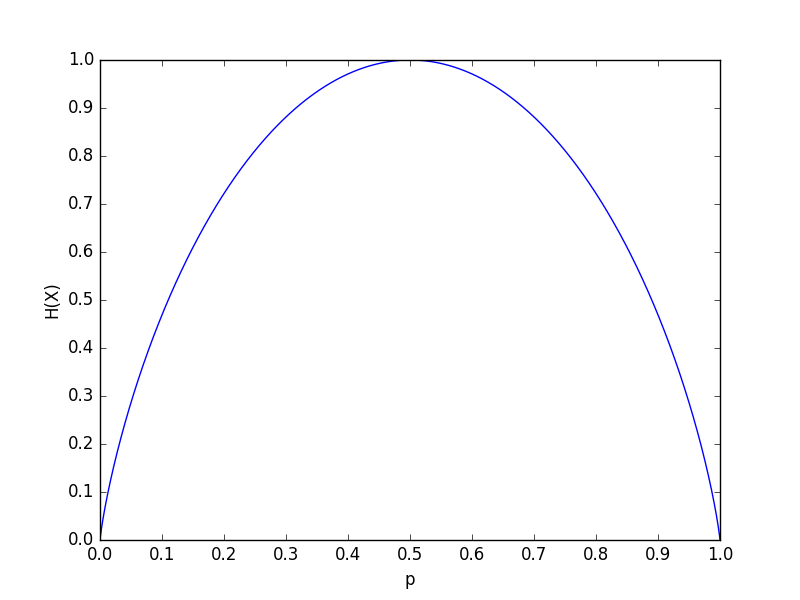
\includegraphics[width=.9\textwidth]{entropy}
\caption{Entropy of $X$ plotted against the value of $p$.}
\label{fig:entropy}
\end{center}
\end{figure}

Due to the fundamentality of the measure, the usage of entropy is ubiquitous throughout science and engineering. For example, in finance, it is extensively used in portfolio selection theory to measure the diversity and risk of the portfolio \cite{entropy-finance}. In civil engineering, it is is a key ingredient in structural optimization design \cite{entropy-civil-eng} - a subfield of optimization that is conserned with improving the design of structures with respect to various specifications (safety, cost, weight etc.). A rather interesting example of application of entropy comes from cognitive neuroscience, where it has been used to characterize different states of consciousness in the brain \cite{entropy-consciousness}.

\subsubsection{Joint and Conditional Entropy}

The \textit{joint entropy} \cite{cover-thomas} of the pair $(X,Y)$ is defined as 

\begin{equation}
H(X,Y) = -\sum_{i=1}^n \sum_{j=1}^m p(x_i,y_j) \log p(x_i,y_j)
\label{eq:cond-etropy}
\end{equation}

This is a direct generalization of entropy to multiple variables. Joint entropy for more than 2 random variables can be defined analogously.

The \textit{conditional entropy} \cite{cover-thomas} of the pair $(X,Y)$ is defined as 

\begin{equation}
H(Y|X) = - \sum_{i=1}^n \sum_{j=1}^m p(x_i,y_j) \log p(y_j|x_i)
\end{equation}

Conditional entropy can be thought of as the amount of uncertainty one has about a random variable $Y$, given that $X$ has already been observed. As a special case, if $X$ and $Y$ are independent, observing $X$ does not reveal anything about $Y$, and $H(Y) = H(Y|X)$.

The  
The entropy of a pair of random variables is the entropy of one plus the conditional entropy of the other \cite{cover-thomas}: 

\begin{equation}
\begin{split}
H(X,Y) & = -\sum_{i=1}^n \sum_{j=1}^m p(x_i,y_j) \log p(x_i,y_j) \\
 	   & = -\sum_{i=1}^n \sum_{j=1}^m p(x_i,y_j) \log p_X(x_i)p(y_j|x_i) \\ 
 	   & = -\sum_{i=1}^n \sum_{j=1}^m p(x_i,y_j) \log p_X(x_i) - \sum_{i=1}^n \sum_{j=1}^m p(x_i,y_j) \log p(y_j|x_i) \\
 	   & = -\sum_{i=1}^n p_X(x_i) \log p_X(x_i) - \sum_{i=1}^n \sum_{j=1}^m p(x_i,y_j) \log p(y_j|x_i) \\ 
 	   & = H(X) + H(Y|X)
\label{eq:chain-rule-entropy}
\end{split}
\end{equation}


\subsubsection{Kullback-Leibler distance}

Let $p_X(x)$ and $q_X(x)$ be two probability mass functions over the support of the random variable $X$. The \textit{relative entropy} or \textit{Kullback-Leibler distance} \cite{cover-thomas} between $p_X(x)$ and $q_X(x)$ is defined as

\begin{equation}
D(p||q) = \sum_{i = 1}^n p(x_i) \log \frac{p_X(x_i)}{q_X(x_i)}
\label{eq:kl-distance}
\end{equation} 

The above quantity is called a distance, because it can be thought of as measuring how far two probability distributions are from each other. Importantly, the relative entropy is non-negative, with inequality exactly when the 2 distributions are equal \cite{cover-thomas}, again corresponding to our intuitive notion of distance. Indeed, when the two distributions are the same, the logarihm in equation \ref{eq:kl-distance} evaluates to 0, which in turn yields a relative entropy of 0. 

However, it must be stressed that since the Kullback-Leibler distance it is not symmetric and does not satisfy the triangle inequality, it is not a formal distance in the mathematically rigorous sense.

\subsubsection{Mutual information}

The \textit{mutual information} \cite{cover-thomas} between the random variables $X$ and $Y$ is given by 

\begin{equation}
MI(X;Y) = \sum_{i=1}^n \sum_{j=1}^m p(x_i,y_j) \log \frac{p(x_i,y_j)}{p_X(x_i)p_Y(y_j)}
\label{eq:mutual-inf}
\end{equation}

An attentive reader might notice that the mutual information is the Kullback-Leibler distance between the joint distribution $p(x,y)$ and the product distribution $p_X(x)p_Y(y)$.

Because the mutual information is just a special case of Kullback-Leibler distance, all the properties that hold for relative entropy must also hold for mutual information. In particular, mutual information must be non-negative and 0 exactly when the random variables $X$ and $Y$ are independent. The latter statement must hold, because if $X$ and $Y$ are independent, then $p(x,y) = p_X(x)p_Y(y)$ by definition. Unlike the general Kullback-Leibler distance, however, the mutual information is symmetric. It follows that the amount of information $X$ has about $Y$ is always equal to the amount of information $Y$ has about $X$. 

Considering mutual information as a special case of Kullback-Leibler distance, it can be intuitively seen as measuring how far the two random variables $X$ and $Y$ are from being independent. Indeed, when the two are completely independent, one would expect that they contain no information about each other, and this is exactly the conclusion that was reached mathematically directly from equation \ref{eq:mutual-inf}.

The picture of mutual information as a distance between two probability distributions yields a straightforward answer to the question: "when is there no information between the two random variables?" However, it does not help in answering the orthogonal question: "when is the information maximized?" To answer the latter, the following identity from \cite{cover-thomas}, which relates mutual information directly to entropy, is of importance: 

\begin{equation}
\begin{split}
MI(X;Y) & = \sum_{i=1}^n \sum_{j=1}^m p(x_i,y_j) \log \frac{p(x_i,y_j)}{p_X(x_i)p_Y(y_j)} \\
		& = \sum_{i=1}^n \sum_{j=1}^m p(x_i, y_j) \log \frac{p(x_i|y_j)}{p_X(x_i)} \\ 
 		& = -\sum_{i=1}^n \sum_{j=1}^m p(x_i,y_j) \log p_X(x_i) +\sum_{i=1}^n \sum_{j=1}^m p(x_i,y_j) \log p(x_i|y_j) \\
 		& = -\sum_{i=1}^n \sum_{j=1}^m p_X(x_i) - \left( - \sum_{i=1}^n \sum_{j=1}^m p(x_i,y_j) \log p(x_i|y_j) \right) \\ 
 		& = H(X) - H(X|Y)
\label{eq:mutual-inf-entropy} 
\end{split}
\end{equation}

Intuitively, using identity \ref{eq:mutual-inf-entropy}, mutual information between random variables $X$ and $Y$ can be thought of as the reduction in the uncertainty of $X$ due to the knowledge of $Y$ \cite{cover-thomas}. Thus, it is maximized when knowing $Y$ completely determines $X$, yielding $H(X|Y) = 0$.  

\subsubsection{Conditional mutual information}

Let $Z$ be a discrete random variable. The \textit{conditional mutual information} \cite{cover-thomas} of the random variables $X$ and $Y$ given $Z$ is defined by 

\begin{equation}
MI(X;Y|Z) = H(X|Z) - H(X|Y,Z)
\end{equation}

Intuitively, the conditional mutual information measures the reduction in the uncertainty of $X$ due to the knowledge of $Y$, given that $Z$ has already been observed. 

Another useful property that will become important in the discussion on partial information decomposition is the \textit{chain rule for information} \cite{cover-thomas}, which expresses the mutual information between a random vector and a random variable in terms of mutual informations between univariate random variables: \footnote{Note that $MI(X;Y,Z)$ means that the mutual information is measured between the random variable X and the random vector (Y,Z). In particular, a semicolon (;) separates the random vectors that the mutual information is measured between (a single random variable is considered a univariate random vector), while a comma (,) separates the random variables in a single random vector.}

\begin{equation}
\begin{split}
MI(X;Y,Z) & = H(Y,Z) - H(Y,Z|X) \\ 
		  & = H(Y) + H(Z|Y) - H(Y|X) - H(Z|Y,X) \\ 
		  & = H(Y) - H(Y|X) + H(Z|Y) - H(Z|Y,X) \\ 
		  & = MI(X;Y) + MI(X;Z|Y)
\label{eq:chain-rule-inf}
\end{split}
\end{equation}

When the information between two random variables is measured in a system with many other dependent variables, conditional mutual information is used to eliminate the influence of the other variables, in order to isolate the two variables of interest \cite{williams-beer}. For example, it has been used to analyse the functional connectivity of different brain regions in schizoprenic patients \cite{brain-cond-inf}.

\subsection{Partial information decomposition}

Mutual information measures the amount of information two random variables, or more generally, two random vectors have about each other. However, it is often worthwhile to ask how much information does an ensemble of input (source) random variables carry about some output (target) variable. 

A trivial solution would be to measure the mutual information between the whole input ensemble considered as a single random vector and the output. However, this would not capture the interactions between the input variables themselves. Moreover, by considering the input ensemble as a single unit, knowledge about how the interactions between specific individual units and the output differ is lost. 

This section introduces \textit{partial information decomposition (PID)} - a mathematical framework for decomposing mutual information between a group of input variables and single source variable.   

\subsubsection{Formulation}

The simplest non-trivial system to analyse that has an ensemble of inputs and a single output is a system with \textit{two} inputs. Given this setup, one can ask how much information does one input variable have about the output that the other does not, how much information do they share about the output, and how much information do they jointly have about the output such that both inputs must be present for this information to exist.

More formally, let $Y$ and $Z$ be two random variables that are considered as sources to a third random variable $X$. By equation \ref{eq:mutual-inf-entropy}, the mutual information between the pair $(Y,Z)$ and $X$ is defined as 

$$MI(X;Y,Z) = H(X) - H(X|Y,Z)$$

The partial information decompositon framework decomposes this mutual information into \textit{unique}, \textit{redundant} and \textit{complementary information} terms. 

Unique information quantifies the amount of information that only one of the input variables has about the output variable. The unique information that $Y$ has about the output $X$ is denoted as $UI(X:Y \setminus Z)$. Similarly, $UI(X:Z \setminus Y)$ denotes the unqiue information that $Z$ has about the target $X$.

As an example, consider table \ref{table:1}, inspired by \cite{pid-synergy}, which depicts the joint distribution of the random vector $(X,Y,Z)$. From the table, it can be seen that the output variable $X$ has 4 equiprobable states, each of which is uniquely specified by the two inputs $Y$ and $Z$. There is some unique information present in both $Y$ and $Z$, because they contain different information about the output $X$ that is not provided by the other input. Indeed, input $Y$ is able to differentiate between the sets $\{0,1\}$ and $\{2,3\}$, while $Z$ discriminates between $\{0, 2\}$ and $\{1,3\}$.

% unique information table
\begin{table}[h!]
\centering
\caption{A joint distribution that provides an example of unique information.}
\begin{tabular}{|c c |c|c|}
	\hline
	Y & Z & X & Pr\\ 
	\hline
	0 & 1 & 0 & $1/4$ \\
	0 & 3 & 1 & $1/4$ \\
	2 & 1 & 2 & $1/4$ \\
	2 & 3 & 3 & $1/4$ \\
	\hline
\end{tabular}
\label{table:1}
\end{table}

Shared information quantifies the amount of information both inputs share about the output variable. It is also sometimes called \textit{redundant} information, because if both inputs contain the same information about the output, it would suffice to observe only one of the input variables. The shared information is denoted as $SI(X:Y;Z)$.\footnote{To be consistent with the the previous section on information theory and \cite{cover-thomas}, the notation used in this thesis for PID terms deviates a little from the one introduced in \cite{bertschinger}. Specifically, a colon (:) is used to partition the set of random variables to a single output (on the left hand side) and a set of inputs (on the right hand side). As before, a semicolon (;) is used to separate the input variables on the right hand side, signifying that these variables are considered to be separate entities, not part of a single random vector.}

Table \ref{table:2}, again inspired by \cite{pid-synergy}, gives a toy example of shared information. The output variable $X$ has 2 equiprobable states, each of which is again uniquely specified by the two inputs $Y$ and $Z$. However, in this example, it would actually suffice to observe only one of the inputs $Y$ or $Z$ to uniquely determine the output. This can easily be verified by noticing that the output $X$ is merely a replication of either input. In other words, one of the input variables is redundant, since the two inputs share all their information about the output.

% redundant information table
\begin{table}[h!]
\centering
\caption{A joint distribution that provides an example of shared sinformation.}
\begin{tabular}{|c c |c|c|}
	\hline
	Y & Z & X & Pr\\ 
	\hline
	0 & 0 & 0 & $1/2$\\
	1 & 1 & 1 & $1/2$\\ 
	\hline
\end{tabular}
\label{table:2}
\end{table}

Complementary or \textit{synergetic} information quantifies the amount of information that is only present when both inputs are considered jointly. The complementary information is denoted as $CI(X:Y;Z)$. 

Table \ref{table:3} depicts the \texttt{XOR}-gate - the canonical example for illustrating the concept of synergy \cite{pid-synergy}. As before, the output $X$ is fully specified by the two inputs $Y$ and $Z$. However, in this case \textit{both} inputs $Y$ and $Z$ must be present for the output to be fully determined, and observing a single input $Y$ would not provide the observer \textit{any} information about the output $X$. Indeed, given a specific value of either $Y$ or $Z$, two equiprobable values for $X$ remain, exactly as was the case before observing none of the inputs. 

% synergy table
\begin{table}[h!]
\centering
\caption{Joint distribution of an \texttt{XOR} function that provides an example of complementary information.}
\begin{tabular}{|c c |c|c|}
	\hline
	Y & Z & X & Pr\\ 
	\hline
	0 & 0 & 0 & $1/4$ \\
	0 & 1 & 1 & $1/4$ \\ 
	1 & 0 & 1 & $1/4$ \\ 
	1 & 1 & 0 & $1/4$ \\ 
	\hline
\end{tabular}
\label{table:3}
\end{table}

It is generally agreed (\cite{williams-beer}, \cite{bertschinger}, \cite{pid-redundant}, \cite{pid-synergy}) that mutual information can be docomposed into the four terms just described as follows:
\begin{equation}
MI(X;Y,Z) = SI(X:Y;Z) + UI(X:Y \setminus Z) + UI(X:Z \setminus Y) + CI(X:Y;Z)
\label{eq:pid}
\end{equation}

The same sources also agree on the decomposition of information that a single variable, either $Y$ or $Z$, has about the output $X$: 
\begin{equation}
\begin{split}
MI(X;Y) = UI(X:Y \setminus Z) + SI(X:Y;Z) \\
MI(X;Z) = UI(X:Z \setminus Y) + SI(X:Y;Z)
\label{eq:pid-yz}
\end{split}
\end{equation}

It is important to note that thus far in this section, no formulas for actually calculating the PID terms have been given, only several logical relationships that such a decomposition should satisfy have been stated. The only computable quantities so far are the mutual information terms at the left hand side of equations \ref{eq:pid} and \ref{eq:pid-yz}, which can be calculated using formula \ref{eq:mutual-inf}. The discussion of computing the specific PID terms is developed in the next section, which is heavily inspired by an intuitive overview of \cite{bertschinger} given in \cite{pid-goal-functions}. 

\subsubsection{Calculating PID terms}

It turns out that the current tools from classical information theory - entropy and various forms of mutual information - are not enough to calculate any of the terms of the PID \cite{williams-beer}. Indeed, there are only 3 equations (\ref{eq:pid}, \ref{eq:pid-yz}) relating to the 4 variables of interest, making the system underdetermined. In order to make the problem tractable, a definition of at least one of the PID terms must be given \cite{bertschinger}.

Taking inspiration from game theory, \cite{bertschinger} were able to provide such a definition for unique information. Their insight was that if a variable contains unique information, there must be a way to exploit it. In other words, there must exist a situation such that an agent having access to unique information has an advantage over another agent who does not possess this knowledge. Given such a situation, the agent in posession of unique information can prove it to others by designing a bet on the output variable, such that on average, the bet is won by the designer.

In particular, suppose there are two agents - Alice and Bob - Alice having access to the random variable $Y$ and Bob having access to the random variable $Z$ from equation \ref{eq:pid}. Neither of them have access to the other player's random variable, and both of them can observe, but not directly modify, the output variable $X$. Alice can prove to Bob that she has unique information about $X$ via $Y$ by constructing a bet on the outcomes of $X$. Since Alice can only directly \textit{modify} $Y$ and \textit{observe} the outcome $X$, her reward will depend only on the distribution $p(X,Y)$. \footnote{Again, for consistency with \cite{cover-thomas}, the probability distributions are denoted with small letters, instead of capital letters as is done in \cite{bertschinger}.} Similarly, Bob's reward will depend only on the distributon $p(X,Z)$. From this, it follows that the results of the bet are \textit{not} dependent on the full distribution $p(X,Y,Z)$, but rather only on its marginals $p(X,Y)$ and $p(X,Z)$.

Let $p = p(X,Y,Z)$ be the original joint probability distribution  that we are interested in computing the PID of, and let $\Delta$ be the set of \textit{all} joint probability distributions of $X$, $Y$ and $Z$. Under the assumption that the unique information depends only on the two marginal distribution of $P$, a set of probability distributions $\Delta_P$ can be defined such that the unique information stays constant for any element in this set. Such a set must consist only of the probability distributions that have the same marginal distributions of the pairs $(X,Y)$ and $(X,Z)$ as $P$. It is defined as follows: 

\begin{multline*}
\Delta_p = \{q \in \Delta: q(X=x, Y=y) = p(X=x, Y=y) \\ 
\text{ and }  q(X=x, Z=z) = p(X=x, Z=z) \text{ for all } x \in X, y \in Y, z \in Z\}
\end{multline*}

Putting the observation that unique information is constant on $\Delta_p$ and equation \ref{eq:pid-yz} together, it becomes apparent that shared information will also be constant on $\Delta_P$. Thus, only complementary information varies when considering arbitrary distribution $q$ from $\Delta_p$. The last observation makes sense intuitively and is to be expected, since "complementary information should capture precisely the information that is carried by the joint dependencies between $X$, $Y$ and $Z$" \cite{bertschinger}. 

Using the chain rule for information (equation \ref{eq:chain-rule-inf}) as well as decompositions \ref{eq:pid} and \ref{eq:pid-yz}, the following identities can be derived: 

\begin{equation}
\begin{split}
MI(X;Y|Z) = UI(X:Y \setminus Z) + CI(X:Y;Z) \\ 
MI(X;Z|Y) = UI(X:Z \setminus Y) + CI(X:Y;Z)
\label{eq:mi-ui-ci}
\end{split}
\end{equation}

Now, if a distribution $q_0 \in \Delta_p$ could be found that yields vanishing synergy, the unique information could be calculated using quantities from classical information theory. Indeed, from equation \ref{eq:mi-ui-ci} it can be seen that when synergy is $0$, the mutual information and unique information terms coincide. However, \cite{bertschinger} prove that a distribution $q_0 \in \Delta_p$ with this property only exists for specific measures of unique, shared and complementary information. They define the suitable measure for unique information as follows:

\begin{equation}
\widetilde{UI}(X:Y \setminus Z) = \min_{q \in \Delta p} MI_q(X;Y|Z)
\label{eq:tilde_ui_y}
\end{equation}

\begin{equation}
\widetilde{UI}(X:Z \setminus Y) = \min_{q \in \Delta_p} MI_q(X;Z|Y)
\label{eq:tilde_ui_z}
\end{equation}

where the subscript $q$ under the mutual information symbol means that the quantity is calculated over the distribution $q$.

Replacing these measures with the corresponding quantities in equations \ref{eq:pid} and \ref{eq:pid-yz}, measures for shared and complementary information can be defined: 

\begin{equation}
\widetilde{SI}(X:Y;Z) = \max_{q \in \Delta_p} MI_q (X;Y) - MI_q(X;Y|Z)
\label{eq:tilde_si}
\end{equation}

\begin{equation}
\widetilde{CI}(X:Y;Z) = MI(X;Y,Z) - \min_{q \in \Delta_p} MI_q(X:Y,Z)
\label{eq:tilde_ci}
\end{equation}

These 4 constrained optimization problems (\ref{eq:tilde_ui_y}, \ref{eq:tilde_ui_z}, \ref{eq:tilde_si}, \ref{eq:tilde_ci}) are all equivalent in the sense that it would suffice to solve only one of these problems and the obtained optimal joint distribution $q$ would produce the optimal value for all the remaining three measures as well. 

\subsubsection{Numerical Estimator}

Bertschinger et al. show that "the optimization problems involved in the definitions of $\widetilde{UI}$, $\widetilde{SI}$ and $\widetilde{CI}$ . . . are convex optimization problems on convex sets" \cite{bertschinger}. A notable property of convex functions is that their local and global minimums coincide, making the optimization problems that involve such functions relatively easy to solve. Indeed, many effictive  algorithms have been developed that solve even large convex problems both efficiently and reliably \cite{boyd}.

"The optimization problems in Lemma 4 can be very ill-conditioned, in the sense that there are directions in which the function varies fast, and other directions in which the function varies slowly." - BROJA. \textcolor{red}{Why is this bad?}
\textcolor{red}{TODO! Consult Dirk on the estimator.}

The numerical estimator takes the approach of solving the optimization problem given in equation \ref{eq:tilde_ci} and then using the resulting distribution $q$ to find the other quantities of interest. The interface of the estimator is rather simple, abstracting away all the details of its inner workings: it takes as input a  probability distribution $p(X, Y, Z)$ and outputs the scalars $MI(X;Y,Z)$, $UI(X:Y \setminus Z)$, $UI(X:Z \setminus Y)$, $SI(X:Y;Z)$ and $CI(X:Y;Z)$. Currently, the estimator is only able to handle discrete distributions. The software is written in Python 3. The convex programming is done in CVXOPT \cite{cvxopt}, while all linear progams are solved using Gurobi \cite{gurobi}. 

\subsection{Ising Model}

In nature, many systems have the property of abruptly transitioning from one state to a completely different state due to some change in the external conditions that they are influenced by. Such a phenomenon, where a system does not change its state smoothly, but rather does it in an all-or-nothing fashion, is called a \textit{phase transition}. A large class of phase transitions, which are of great practical importance, can be thought of as shifts from an ordered state to a disordered one, or vice versa. A canonical example of this phenomenon comes form condensed matter phycics, where matter transitions quickly from a fairly ordered solid state to a relatively less organized liquid state when temperature passes a specific threshold.\cite{inf-flow-ising-commentary}

In this section, one of the simplest models that undergoes a phase transition - the Ising model - is introduced. The Ising model can be characterized as a dynamical complex system, because it has many parts whose simple local interactions give rise to a complex global phenomenon in the form of the phase transition. 

\subsubsection{Ferromagnetism}

Before introducing the Ising model, a short overview of a phycsical mechanism that it is modelling - ferromagnetism - is in order. This is done in this subsection, which is based on \cite{memory-systems-cache-ram}.

Electrons in a material have magnetic moments, caused by their spins, which can be in either one of two states. These small magnetic properties of individual electrons do not usually yield a global net magnetization of the material, because the electron in the atoms often come in pairs of opposite spin states, cancelling each other out. However, in ferromagnets, there are many unpaired electrons, which line up with each other, producing a region called a \textit{domain}. While the magnetic field is strong within the domain, the material is still unmagnetized because the many domains themselves are oriented randomly with respect to one another. A characteristic property of a ferromagnetic materials is that even a rather weak external magnetic field can can cause the magnetic domains to line up with each other. When this happens, the material is said to be magnetized. Importantly, in the case of a ferromagnet, the material will remain magnetized even if the influencing external field is removed. 

The stability of the magnetization is also dependent on the temperature of the substance. Intuitively, at high temperatures, the atoms in the substance become agitated and start to vibrate. This thermal oscillation breaks the alignment of the spins and the material demagnetizes. This is yet another example of a phase transition in which an ordered, magnetized system abruptly changes it state to an unordered one. The critical temperature at which this transition happens is called the \textit{Curie temperature}.

\subsubsection{Model} 

The Ising model, first conceived by Wilhelm Lenz in 1920 \cite{ising-history}, is a mathematical model of ferromagnetism. The model abstracts away the rather complex details of atomic structures of magnets, consisting simply of a discrete lattice of cells or sites, denoted as $s_i$, each of which has an associated binary value of either -1 or +1. Conceptually, the lattice can be thought of as a physical material, where the sites roughly represent the unpaired electrons of its atoms. The binary value of each site intuitively corresponds to the direction of the electron's spin. A value of -1 means that the spin is considered to point "down", otherwise it is said to be pointing "up". A given set of spins, denoted as $\boldsymbol{s}$ (without the subscript), is called the \textit{configuration} of the lattice. \cite{statistical-mechanics}

The magnetization of a configuration $\boldsymbol{s}$ of an Ising model with a lattice of $N$ sites is given by 

\begin{equation}
M(\boldsymbol{s}) = \frac{1}{N} \sum_{i=1}^N s_i
\label{eq:magnetization}
\end{equation}

From equation \ref{eq:magnetization}, it can bee seen that the absolute magnetization is small when the number of "up" spins is roughly the same as the number of "down" spins. On the other hand, if all the spins point in the same direction, the absolute magnetization is at it maximum, having a value of 1. This is indeed analogous to the mechanism in play in physical ferromagnets, as described earlier. 

The dynamics of the Ising model stem from the fact that the specific spin configurations of the Ising model are random variables. The probability of a configuration $\boldsymbol{s}$ at thermal equilibrium is given by the Boltzmann distribution: 

\begin{equation}
P_\beta(\boldsymbol{s}) = \frac{e^{-\beta E(\boldsymbol{s})}}{\sum_{\boldsymbol{s}} e^{-\beta E(\boldsymbol{s})}}
\label{eq:boltzmann-dist}
\end{equation}

where $E(\boldsymbol{s})$ denotes the \textit{energy} associated with the configuration $\boldsymbol{s}$, and $\beta = \frac{1}{k_B T}$ where $T$ is the temperature and $k_B$ is the Boltzmann constant. Thus, $\beta$ is proportional to the inverse temperature of the system.  

Thus, the probability of a configuration $\boldsymbol{s}$ depends on 2 unrelated quantities: the internal energy of the configuration under discussion, and the temperature. Two observations that stem from equation \ref{eq:boltzmann-dist} are of importance. First, the lower the energy $E(\boldsymbol{s})$ of a configuration $\boldsymbol{s}$, the higher its probability. Second, the higher the temperature $T$ (or equivalently, the lower the parameter $\beta$), the more diffuse the distribution becomes. The latter mathematical property models the physical fact that at high temperatures, the thermal oscillation of the atoms break the alignment of the spins, demagnetizing the material. 

Energy is a central quantitiy that is associated with almost any model in physics. In the Ising model, energy is given by the Hamiltonian

\begin{equation}
E(\boldsymbol{s}) = - \sum_{\langle ij \rangle} \epsilon s_i s_j - H \sum_{i=1}^N s_i
\label{eq:ising-hamiltonian}
\end{equation}

where the first sum is over all different neighboring spins, $\epsilon$ is the interaction strength between adjacent spins, and $H$ denotes the strength of an exetrnal magnetic field. The latter two quantities are given constants that are specified by the properties of the magnetic material and the external environment of the system, respectively.

Often, the model is simplified even further. In particular, the external magnetic field interacting with the lattice is omitted, and the interaction strength between pairs of nearest neighbors is fixed to be equal to the Boltzmann constant $k_B$, so that they cancel each other out in equation \ref{eq:ising-hamiltonian} and $\beta$ becomes exactly the inverse temperature $\frac{1}{T}$. After incorporating these assumptions into the model, the energy of a configuration $\boldsymbol{s}$ simplifies to 

\begin{equation}
H(\boldsymbol{s}) = - \sum_{\langle ij \rangle} s_i s_j
\label{eq:ising-hamiltonian-simple}
\end{equation}

From equation \ref{eq:ising-hamiltonian-simple}, it can be seen that the spins in the Ising model directly interact with only their nearest neighbors. Moreover, since there is a minus sign in front of the sum, lower energy (and thus, a higher probability) is achieved when neighboring spins take on the same value, as this yields a positive product. It can be intuitively thought as if the spins are intrinsically trying to align with their neighbors, and the temperature of the system quantifies the amount of prohibition that prevents them from doing so. 

There are many questions one could ask about the dynamics of the Ising model, but perhaps the most interesting and most extensively studied is the following: how does the magnetization of the lattice change with temperature? Since for a fixed value of $\beta$, the lattice configurations are random variables, an \textit{expectation} of the magnetization must be found, using the following formula:

\begin{equation}
\langle M \rangle_\beta = \sum_{\boldsymbol{s}} M_\beta(\boldsymbol{s}) P_\beta(\boldsymbol{s})
\label{eq:expected-mag-ising}
\end{equation}

By saying that there is a phase transition in the Ising model, what is meant is that there exists a critical temperature $T_c$ such that for temperatures $T > T_c$, the expected magnetization given by equation \ref{eq:expected-mag-ising} is 0 (or quickly approaches zero if $T$ is near $T_c$). Conversely, if $T < T_c$, the absolute magnetization is 1. Ernst Ising himself proved that there is no sponatneous magnetization and therefore, no phase transition in the 1-dimensional Ising model \cite{Ising1925}. On the other hand, in 1944, Lars Onsager showed \cite{lars-onsanger} that the 2-dimensional Ising model with a square lattice does undergo a phase transition in the absence of an external magnetic field. Furthermore, he gave the exact value of the parameter $\beta$ at which the swift order-disorder transition takes place. For higher dimensional Ising models, no analytic solution for the phase transition exists. 

\subsection{Elementary Cellular Automata}

Elementary cellular automata (ECA) are discrete dynamical complex systems that consist of a 1-dimensional array of cells, each of which has an associated binary value. Every automaton is uniquely defined by its rule table - a function that maps the value of a cell to a new value based on the cell's current value and the values of its 2 immediate neighbors. Since each rule table has a corresponds to a unique 8-bit binary number, there are only $2^8 = 256$ elementary cellular automata in total, each of which is associated with a unique decimal number from 0 to 255. Figure \ref{fig:eca-rule-table} gives an example of one such rule table, where the top row represents the state's all possible local neighborhoods and the bottom row represents the center state's new value. For example, one can infer from the table that if a cell has a value of 0 (white) while both of its neighbors have a value of 1 (black), then this cell will retain its value after the function has been applied. 

\begin{figure} [!h]
\begin{center}
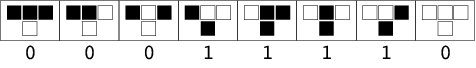
\includegraphics[width=0.8\textwidth]{eca-rule-example}
\caption{Rule 30 \cite{weisstein-eca}.}
\label{fig:eca-rule-table}
\end{center}
\end{figure}

Elementary cellular automata can be simulated in time by simultaneously applying the update rule to each cell in the 1-dimensional array, producing a 2-dimensional plot where the vertical axis represents time. The result of evolving the rule illustrated in figure \ref{fig:eca-rule-table}, given an initial lattice configuration of all white cells except the center, can be seen in figure \ref{fig:eca-rule-dynamics}. Notably, the figure shows that the evolution of the dynamics is rather non-trivial. Indeed, cellular automata are interesting precisely because despite their simplicity, the patterns that emerge as a function of the rule table and the initial configuration can be quite complex. For example, elementary cellular automata have been shown to be capable of generating random numbers \cite{eca-random-gen}, modelling city traffic \cite{eca-city-traffic}, and perhaps most astonishingly, simulating any Turing machine \cite{eca-universal}. On the other hand, there exists a lot of rules which quickly converge into an uninteresting homogeneous or repetitive state. 

\begin{figure} [!h]
\begin{center}
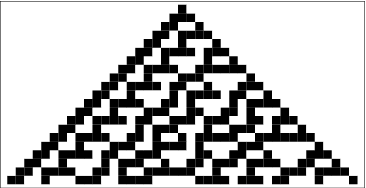
\includegraphics[width=0.8\textwidth]{eca-dynamics-example}
\caption{A space-time diagram of the evolution of rule 30 \cite{weisstein-eca}.}
\label{fig:eca-rule-dynamics}
\end{center}
\end{figure} 

Because the set of all elementary cellular automata is rather diverse, consisting of both computationally interesting as well as uninteresting rules, it would make sense to try to group them based on the apparent complexity of their behvaiour. In the seminal paper Universality and Complexity in Cellular Automata \cite{wolfram-classification}, Stephen Wolfram does just that. After qualititively analysing the global structures that the different rules give rise to given random initial states, he proposes a classification scheme that partitions all elementary cellular automata into four classes. The proposed classes are as follows:

\begin{itemize}
\item Class 1: Cellular automata which converge to a homogeneous state. For example, rule 0, which takes any state into a 0 state, belongs to this class.
\item Class 2: Ceullar automata which converge to a repetitive or periodic state. For example, rule 184, which has been used to model traffic, belongs to this class.
\item Class 3: Cellular automata which evolve chaotically. For example, rule 30, which Mathematica uses as a random number generator \cite{NKS}, belongs to this class.
\item Class 4: Cellular automata in which persistent propagating structures are formed. For example, rule 110, which is capable of universal computation, belongs to this class. It is conjectured that other rules in this class are also universal. 
\end{itemize}

\newpage
\section{Related Work} 

This chapter gives a brief overview of prior work closely related to this thesis. The first section introduces previous work on analysing complex systems that undergo a phase transition, such as the Ising model, with information-theoretic tools. The second section focuses on related work that analyse elementary cellular automata.    

\subsection{Phase transitions}

There is a large body of previous work in applying information theory to analyse dynamical complex systems that undergo phase transitions. Specifically, it has been shown that mutual information and other related information-theoretic measures peak at the critical point where the systems undergo an order-disorder transition. Such is the case for several mathematical models like random boolean networks \cite{lizier-rand-bool-nets} and Vicsek's self-propelled particle model \cite{mi-swarms}. 

As for real-world systems, \cite{mi-financial-markets} measured mutual information between pairs of selected stocks and found that the peaks in information take place around known market crashes. To better understand phase transitions in cognitive behaviours, \cite{mi-go} analysed mutual information between successive moves in the game of Go as a function of players' skill level. They found that information peaks around the transition from amateur to professional, "agreeing with other evidence that a radical shift in strategic thinking occurs at this juncture" \cite{mi-social-systems}. 

Particularly relevant to the work at hand is the information-theoretic analysis of the Ising model. It has been analytically shown that in a 2-dimensional Ising model, the mutual information between joint states of two spin systems peaks at the critical temperature \cite{mi-ising-analytic}. \cite{barnett-ising} show empirically that mutual information measured between pairs of neighboring spins peaks at the phase transition. In the current thesis, this result is replicated and extended by also measuring the decomposition terms of this mutual information. \cite{barnett-ising} further discover that another related quantity called transfer entropy, a directed measure that quantifies the transfer of information between two stochastic processes, peaks strictly in the disorder phase \textit{before} the phase transition. 

\subsection{Elementary cellular automata}

Not directly related to this thesis, but contextually rather relevant are various works that have made use of information theory to quantitatively validate long-held hypothesis about information processing in elementary cellular automata. In \cite{active-inf-storage}, Lizier et al. found quantitative evidence that specific structures in elementary cellular automata called blinkers and background domains are "dominant information storage processes in these systems." In another closely related paper \cite{local-transfer-entropy-ca}, the same authors conclude that "local transfer entropy provides the first quantitative evidence for the long-held conjecture that the emergent traveling coherent structures known as particles . . . are the dominant information transfer agents in cellular automata."

Of particular interest to this thesis is the work done in \cite{multi-inf-ca}, in which the behaviour of multi-information, a generalization of mutual information to multible variables, in elementary cellular automata was studied. It was found that while it could be possible to establish a classification of cellular automata rules based on this measure, it would not correspond with Wolfram's 4 classes. This is because multi-information failed to discriminate between all pairs of Wolfram's classes except between classes I and IV.

\newpage
\section{Methods}

This chapter describes the approaches taken in this thesis to analyse the complex systems in terms of partial information decomposition. The first section is devoted to motivating the use of computational simulations in investigating the Ising model, as well as to an overview of a specific algorithm used to carry out such simulations in the current dissertation. The second and third sections of this chapter desribe in detail how the PID estimator is utilised to measure the information distribution in the Ising model and elementary cellular automata, respectively. To ensure reproducibility of the results, the exact values of all the parameters of the experiments are given. 

\subsection{Numerical simulation of the Ising model}

In theory, finding the expected magnetization of the Ising model at a given temperature $T$ is trivial. According to equation \ref{eq:expected-mag-ising}, one simply has to enumerate all lattice configurations, multiply their probabilities by their magnetizations, and sum the products. The problem arises in the very first part - doing an exhaustive search through all lattice configurations. The number of possible configurations of a lattice of size $N$ is $2^N$, meaning that the number of configurations increases exponentially in the size of the lattice. Therefore, the sum in equation \ref{eq:expected-mag-ising} is intractable for even rather modest sized lattices. This is of course a more general problem that is not only present when calculating the expected magnetization, but rather appears in any task where one has to deal with expectations in the Ising model. For example, in this thesis, 
the average mutual informaton between the neighboring sites at each temperature point is of interest. Unable to derive it anlytically, one must resort to simulating the dynamics of the model. 

Because enumerating all possible configurations is intractable, a more clever solution must be found. One way to \textit{approximate} the average quantities is to draw many samples (spin configurations) from the Boltzmann distribution and calculate the quantities of interest on these configurations, taking their mean in the end. If the configurations are drawn in proportion to their probabilites given by equation \ref{eq:boltzmann-dist}, the mean of the quantity of interest will become increasingly closer to the true expectation as the sample size increases. Glauber dynamics, an instance of a more general class of algorithms called Markov Chain Monte Carlo methods, allows one to iteratively draw samples from the Boltzmann distribution according to their probabilities.

The Glauber dynamics method works as follows. First, an initial lattice configuration is generated arbitrarily (as demonstrated in the next section, some clever tricks in choosing the initial configuration can be done, however). Then, iteratively, a site is chosen uniformly at random from the lattice, and the spin associated with this site is flipped. The resulting configuration with a single flipped spin is either accepted or rejected. The probability of acceptance is given by equation \ref{eq:glauber-accept-prob}, where $\boldsymbol{s}$ and $\boldsymbol{s_n}$ denote the old and new lattice configurations, respectively, $T$ stands for temperature and $\Delta E(\boldsymbol{s} -> \boldsymbol{s_n}) = E(\boldsymbol{s}) - E(\boldsymbol{s_n})$ is the difference between the energies of the two successive configurations. For a more compact overview, a pseudocode for a single iteration of Glauber dynamics is given in algorithm \ref{alg:glauber-update}.

\begin{equation}
P(\boldsymbol{s} -> \boldsymbol{s_n}) = \frac{1}{1 + e^\frac{\Delta E(\boldsymbol{s} -> \boldsymbol{s_n})}{T}}
\label{eq:glauber-accept-prob}
\end{equation}

\begin{algorithm}
\textbf{Input:} A lattice configuration $\boldsymbol{s}$ \\
Choose a random site from the lattice\;
Flip the spin associated with the chosen site to obtain a configuration $\boldsymbol{s}_n$\;
Calculate the energy difference: $\Delta E(\boldsymbol{s} -> \boldsymbol{s_n}) = E(\boldsymbol{s}) - E(\boldsymbol{s_n})$\;
Generate a random number $x$ uniformly at random within the range [0, 1]\;
\eIf{$x \leq P(\boldsymbol{s} -> \boldsymbol{s_n})$}{
	\Return $\boldsymbol{s_n}$;  \Comment{accept the new configuration $\boldsymbol{s_n}$ by returning it}
}{
	\Return $\boldsymbol{s}$;  \Comment{reject $\boldsymbol{s_n}$ by returning $\boldsymbol{s}$}
}
\caption{A single iteration of Glauber dynamics}
\label{alg:glauber-update}
\end{algorithm}

There are two noteworthy additions to the naive algorithm \ref{alg:glauber-update} that must be discussed. First, to uncorrelate the samples, many potential spin flips are considered before a sample is actually drawn, meaning that not every lattice configuration returned by algorithm \ref{alg:glauber-update} is considered as a sample, but rather every $L$-th. The parameter $L$ is a called the $lag$. This procedure is illustrated in algorithm \ref{alg:glauber-update-lag}. Notice that indeed, all the intermediate configurations on line $3$ are discarded,  only the $L$-th configuration is eventually returned. Second, in order to avoid biasing the initial samples towards the random starting configuration, the very first samples are discarded. The number of initial disposable samples is referred to as the \textit{burn in period}. The entire simulation algorithm with Glauber dynamics, along with the random initialization of the lattice, burn-in period and lag, is illustrated in algorithm \ref{alg:glauber-full}.

\begin{algorithm}
\textbf{Input:} A lattice configuration $\boldsymbol{s}$ and lag $L$ \\
\For{$i = 1 ... L$} {
	$\boldsymbol{s}$ = Run algorithm \ref{alg:glauber-update} on input $\boldsymbol{s}$\;
}
\Return $\boldsymbol{s}$\;
\caption{A single Glauber dynamics update, which consists of $L$ spin-flip attempts}
\label{alg:glauber-update-lag}
\end{algorithm}

\begin{algorithm}
\textbf{Input:} Burn-in period $B$, lag $L$, and the number of samples to draw $N$ \\ 
Initialize a random lattice configuration $\boldsymbol{s}$\;

\For{$i = 1 ... B$} {  
	$s$ = Run algorithm \ref{alg:glauber-update-lag} on input $s$ and $L$\;
}

set \textit{samples} to empty list  \Comment{List to save the sampled configurations to}\\
\For{$i = 1 ... N$} {
	$s$ = Run algorithm \ref{alg:glauber-update-lag} on input $s$ and $L$\;
	save configuration $\boldsymbol{s}$ to \textit{samples}\;
}

\Return \textit{samples}
\caption{The full Glauber dynamics algorithm}
\label{alg:glauber-full}
\end{algorithm}

When implementing the Ising model with a finite lattice, one also has to decide how are the neighbors for the sites on the edges of the lattice chosen. For example, if a site is on the right edge of the lattice, it does not have an immediate right-hand neighbor. There are two common way to deal with this complication. First, \textit{periodic boundary conditions} can be used, in which the lattice "wraps around" itself, such that the sites on one edge of the lattice have as neighbors sites on the opposite edge, yielding all sites to have the same number of neighbours no matter their position on the lattice \cite{spin-models-thesis}. Second, the sites on the edges of the lattice can be made to have only their usual immediate neighbors, so that sites on the edges have fewer neighbors than sites at the center of the lattice \cite{spin-models-thesis}. In this case, the model is said to have \textit{free boundary conditions}.

\subsection{Methodology for analysing the Ising model}

To estimate the PID terms in the Ising model, a 2-dimensional model with Glauber dynamics, periodic boundary conditions and a square lattice of size 128x128 was simulated. A single simulation consisted of a burn-in period of $10^4$ updates, following $10^5$ updates from which the samples were gathered. As in \cite{barnett-ising}, "each update comprised $L$ (potential) spin-flips according to Glauber transition probabilities", where $L$ is the size of the lattice. In other words, the model was simulated according to algorithm $\ref{alg:glauber-full}$ with $B=10^4$, $N=10^5$ and $L=128\times128$. This procedure was performed at 102 temperature points spaced evenly over the interval [2.0, 2.8], which encloses the theoretical phase transition at $T_c \approx 2.269$. 

The obtained $10^5$ lattice configurations at each temperature  point were subsequently used to construct the probability distributions that the PID estimator takes as input. 100 sites were chosen uniformly at random at the beginning of the simulation, and they stayed the same for all temperature points. For each site, the relative frequency of its local neighborhood (the site itself along with 4 of its neighbors) was measured, yielding a total of 100 joint probability distributions of 5 random variables per temperature point. An example of one such distribution at temperature $T \approx 2.119$ is given by table 2, where the first random variable $C$ represents the center site, and the following 4 random variables represent its immediate neighbors. For example, the last row of the table illustrates that the configuration where all the spins point upwards at a specific location on the lattice has a probability of $0.776$, meaning that is appears approximately $0.776 \times 10^5 = 77 600$ times out of a total of $10^5$ configurations sampled. The high probability of all aligned spins is to be expected, since the samples are taken while the Ising model is in the ordered, low temperature resigme.

% synergy table
\begin{table}[h!]
\centering
\caption{Joint probability distribution of a random site and its 4 neighbors at temperature $T \approx 2.119$. The column labels represent the location of the sites with respect to the neighboring center (C) site: upper (U), right (R), down (D), left (L).}
\begin{tabular}{c c c c c c}
	\hline
	C & U & R & D & L & Pr\\ 
	\hline
	-1 & -1 & -1 & -1 & -1 & 0.004 \\
	-1 & -1 & -1 & -1 & 1 & 0.002 \\
	-1 & -1 & -1 & 1 & -1 & 0.003 \\
	-1 & -1 & -1 & 1 & 1 & 0.003 \\
	.. & .. & .. &  .. & .. & .. \\
	1 & 1 & 1 & -1 & 1 & 0.035 \\
 	1 & 1 & 1 & 1 & -1 & 0.033 \\
 	1 & 1 & 1 & 1 & 1 & 0.776 \\
 	\hline
\end{tabular}
\label{table:4}
\end{table}

Having created $100$ probability distributions for each of the $102$ temperature points, it remains to feed the distributions into the PID estimator for analysis. However, this can not be done naively with the current setup, as the estimator works with probability distributions of 3 random vectors only, where one of them is thought of as an output and the remaining as inputs. Thus, the distributions of the same form as the one in table \ref{table:4} must be reconfigured such that they are understood by the estimator, i.e. it must be decided how are neighboring sites paritioned into 2 sets of inputs and an output. Two different setups were considered. First, the center site was taken to be the output, and only 2 neighbors were chosen without repetitions uniformly at random (out of the possible set of 4 neighbors) as inputs. Second, the center was again considered as an output, but in this experiment all 4 neighbors were taken into consideration as inputs: the full set of neighbors was randomly partitioned into 2 disjoint pairs, such that each pair was a 2-dimensional random vector. After estimating the PID terms, an arithmetic mean across the sites was taken at each temperature point, yielding 102 average PID vectors, one for each temperature point. 

Due to the randomness present in the Glauber dynamics and in choosing the $100$ sites from the lattice for analysis, the results may vary across different runs. To gain more confidence in the results, the whole experiment described above (simulating the Ising model, choosing 100 random sites for analysis, estimating the PID of the local neighborhood of the sites) was repeated 8 times and the results averaged. In the very first run, each initial spin configuration was initialized randomly at each temperature point as in line 2 of algorithm \ref{alg:glauber-full}, and the configuration that was arrived at after the burn in period of $10^4$ updates was saved. For subsequent 7 runs, the very first lattice configuration for temperature point $T_i$ was chosen to be equivalent to the saved lattice configuration from the very first run at temperature point $T_i$. After doing the first run separately to obtain the initial configurations, the 7 remaining simulations to gather the relevant lattice configurations were run for 8 days on 41 computing nodes in parallel in the EENet computer cluster.

\subsection{Methodology for analysing elementary cellular automata}

The average information distribution was estimated in all 88 inequivalent elementary cellular automata. \footnote{While there are 256 different rules in total, some of them are computationally equivalent. In particular, exchanging the roles of black and white in the rule table and reflecting the rule through a vertical axis does not change the computational capabilities of the automaton. Not considering rules that are equivalent under these transformations yields 88 rules that are of interest.} To gather the probability distributions for the PID estimator, 88 automata with $10 000$ cells were simulated for $1000$ time steps using periodic boundary conditions. For each automaton, a random initial configuration was generated, such that each cell at timestep $t=0$ was associated with a value taken uniformly at random from the set $\{0,1\}$.

The input pair was taken to be the cell's 2 neighbors (considered as a single random vector) and the cell itself at timestep $t$, while the output was the cell's value at the next timestep $t+1$. This is indeed a logical setup to use, as it ensures that the input set contains all the variables that the output is a function of. Using these random variables, a single distribution was generated for each rule. Note that this differs from the methodology that was used in the case of the Ising model, where only a subset of the sites was chosen for analysis, yielding 100 different distributions for each temperature point. 

Because the emergent dynamics of a cellular automaton depend on the initial configuration of the lattice, the above experiment (generating initial configurations for each of the 88 automata, simulating the dynamics and generating the distribution that is fed into the estimator) was repeated 5 times, after which the resulting 5 PIDs of each rule were averaged.  

\newpage
\section{Results}

This chapter provides the main results of the thesis. The focus of the first section is on the Ising model, while the second concentrates on elementary cellular automata. 

\subsection{Ising model}

The first subsection of this section is dedicated to measuring the order parameter (magnetization) of the Ising system to validate the simulation methodology. The results obtained from measuring the partial information decomposition terms in models with various lattice sizes are given in the two subsequent sections.

\subsubsection{Phase transition} 

To gain confidence that the Ising model simulations behave as expected, the average absolute magnetization of the 8 runs was measured. The resulting plot can be seen in figure \ref{fig:ising-128-mags}. The phase transition is clearly present, and the critical temperature is around the theoretically correct value of $T_c \approx 2.269$, as given by Onsager \cite{lars-onsanger}. At temperatures $T > T_c$, the magnetization of the Ising model is near 0, while at temperatures $T < T_c$, the absolute magnetization quickly approaches 1 as $T$ decreases. This agrees with previous practical and theoretical research works conducted on the Ising model, thus validating that the simulation is done correctly.

\begin{figure} [h]
\begin{center}
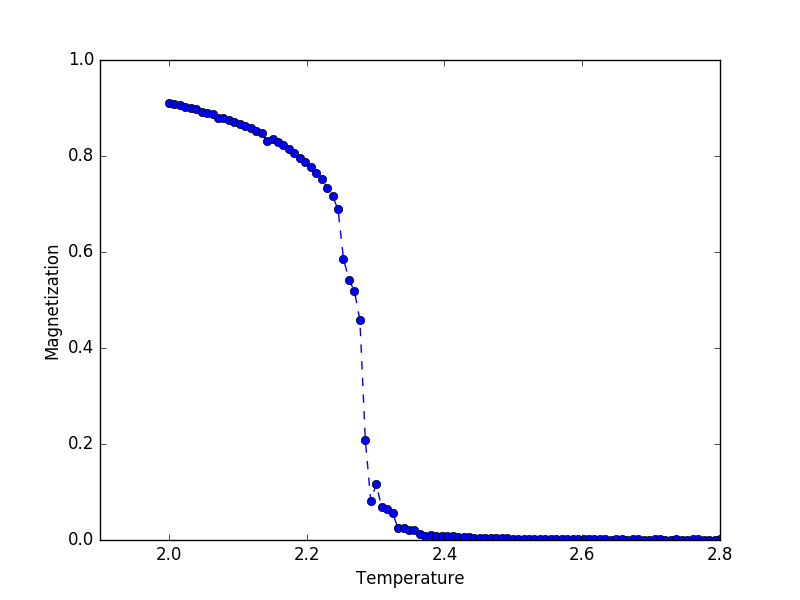
\includegraphics[width=.9\textwidth]{ising-128-mags}
\caption{Average absolute magnetization of a 128x128 lattice Ising model evaluated at 102 temperature points spaced evenly over the interval [2.0, 2.8].}
\label{fig:ising-128-mags}
\end{center}
\end{figure}

\subsubsection{PID on 128x128 Ising model}

In figure \ref{fig:ising-128-pid-2-nbs}, the information-theoretic functionals of the Ising model can be observed, where the mutual information is measured between a sites and their 2 random neighbours. Notice that the information is given in nats, meaning that the base of the logarithm in equation \ref{eq:mutual-inf} is taken to be $e$. 

\begin{figure} [h!]
\begin{center}
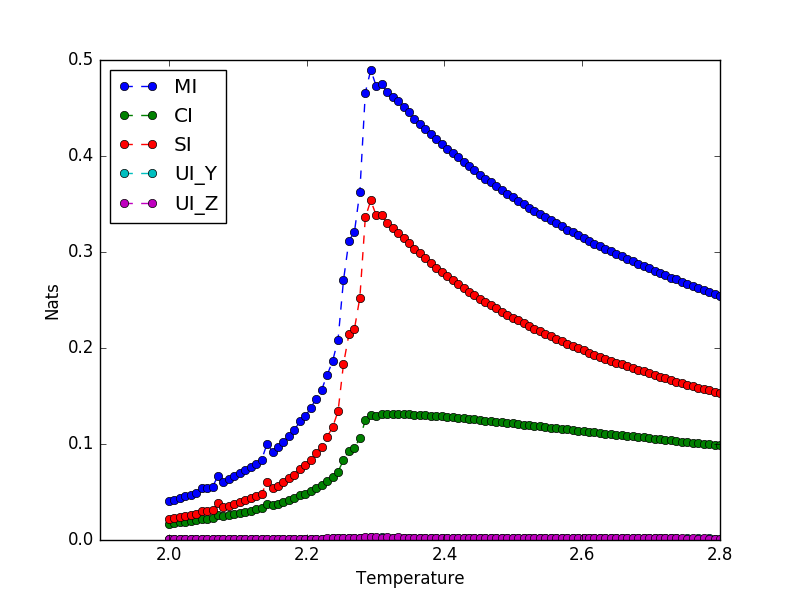
\includegraphics[width=.9\textwidth]{ising-128-pid-2-nbs}
\caption{Average mutual information and PID terms (with 2 random neighbors considered as inputs) of a 128x128 lattice Ising model evaluated at 102 temperature points spaced evenly over the interval [2.0, 2.8].}
\label{fig:ising-128-pid-2-nbs}
\end{center}
\end{figure}

From the figure, it can be seen that mutual information peaks around the phase transition (more precisely, at $T \approx 2.293$) - a phenomenon that agrees with previous work, confirming that the method of estimating the information-theoretic terms used in this thesis works as expected. In addition, since in the experiment under discussion the mutual information was measured between a site and 2 of its neighbors, as opposed to measuring it between 2 neighboring sites only (as was done in \cite{barnett-ising}), it would be reasonable to expect the resulting mutual information to be higher in the current experiment. Indeed, two neighbors should have more information about their center site than a single neighbor has. In \cite{barnett-ising}, the mutual information between 2 neighboring sites (the quantity $I_{pw}$ in the paper) is observed to achieve a maximum value of less than $0.3$. In agreement with intuition, the blue graph representing mutual information in figure \ref{fig:ising-128-pid-2-nbs} achieves a peak value of just under $0.5$.

Looking at the partial information decomposition of the Ising model in figure \ref{fig:ising-128-pid-2-nbs}, one can see that that the non-zero terms peak around the phase transition, just as mutual information itself. Visually, the shared information curve follows the mutual information graph almost exactly, with the expection of being shifted downwads about $1.5$ nats at every temperature point. The synergetic information term is more interesting. It peaks slightly before mutual information does, in the disorder phase at $T \approx 2.333$. In addition, its overall behaviour also deviates from that of mutual information, with the graph being quite a bit flatter, not exhibiting a sharp peak. Both of the unique information terms are rather uninteresting, as their values are essentially zero at every temperature point under consideration. 

Shared information is the most dominant of the partial information decomposition terms in figure \ref{fig:ising-128-pid-2-nbs}, meaning that there is an unproportional amount of redundancy in the system. This is to be expected, as the neighbors of the center site are directly influencing the latter to take on the same value as them, and vice versa. Thus, reasoning by transitivity, a neighboring site $A$ tries to orient its spin to be parallel to the center spin, and similarly, the center site tries to align its spin such that it points in the same direction as the spin of another neighbor $B$. Because $A$ and $B$ are actively trying to make their spins parallel to each other through the influence of the center site, it is not unreasonable to assume that if the spin of one neighbor is known, the spin of the other neighor is also likely to be that same value. 

The unique information terms are always near 0, no matter which neighbor is considered. First, it is reasonable that both of the unique information terms are identical, as the neighbors are chosen randomly. Second, the fact that there is no unique information in the system is intuitively plausible, because the interactions between the spins are completely symmetric. As for the behaviour of synergetic information, the author has no intuitive explanation for the observed pheonomena. 

\begin{figure} [h]
\begin{center}
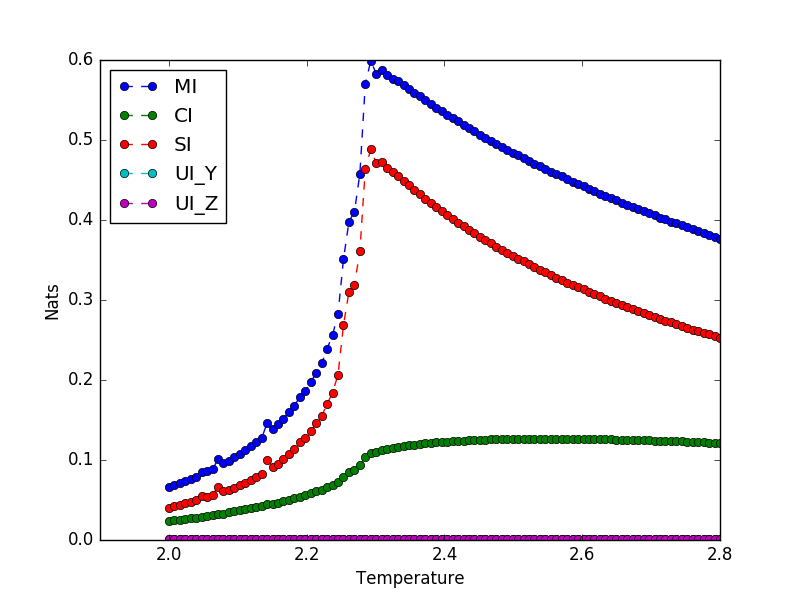
\includegraphics[width=.9\textwidth]{ising-128-pid-4-nbs}
\caption{Average mutual information and PID terms (with all random neighbors considered as inputs) of a 128x128 lattice Ising model evaluated at 102 temperature points spaced evenly over the interval [2.0, 2.8].}
\label{fig:ising-128-pid-4-nbs}
\end{center}
\end{figure}

In figure \ref{fig:ising-128-pid-4-nbs}, the results of measuring information-theoretic functionals between the center sites and all of their neighbors are illustrated. As expected, the mutual information term increases in value (about $1$ nat) compared to figure \ref{fig:ising-128-pid-2-nbs}, because considering all 4 of the sites that interact with the center site, as opposed to just 2, should reduce the amount of uncertainty one has about the center. Further inspection shows that the PID term responsible for the increased mutual information is shared information. The complementary and unique information terms have roughly the same values in both experiments. Specifically, at all temperature points, unique information terms are $0$ and synergetic information varies around $0.1$ nats. 

An unanticipated difference between the first and second experiment is that when all neighbors are considered, the synergetic information term is flatter than before and peaks even deeper in the disorder phase, at temperature $T \approx 2.554$, while shared information does not change its maximum point across the 2 experiments. The former observation is of great importance and could have many practical applications. Its implications are thoroughly examined in the discussion section. 

\subsubsection{PID on 64x64 Ising model}

\begin{figure} [h]
\begin{center}
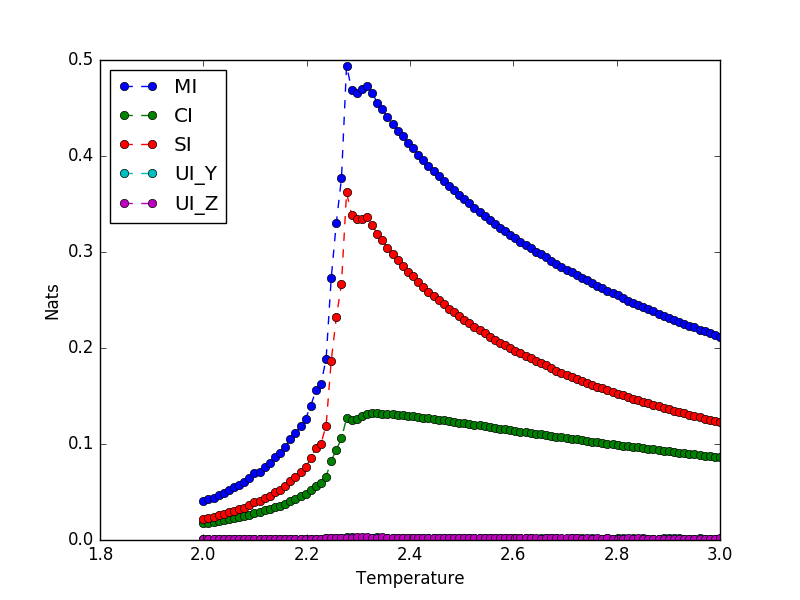
\includegraphics[width=.9\textwidth]{ising-64-pid-2-nbs}
\caption{Average mutual information and PID terms (with 2 random neighbors considered as inputs) of a 64x64 lattice Ising model evaluated at 102 temperature points spaced evenly over the interval [2.0, 3.0].}
\label{fig:ising-64-pid-2-nbs}
\end{center}
\end{figure}

To confirm that the observed phenomena are not specific to a lattice of size 128x128, but are general characteristics of the computational properties of the Ising model, the simulations were repeated with a smaller, 64x64 lattice. The experimental setup was analogous to the one used in the previous experiments, with the exception that the measurments were averaged over 6 different runs (instead of 8) and for each run, 50 different random sites were chosen for PID analysis (instead of 100). The simulations were run on 102 temperature points spaced evenly over the interval [2.0, 3.0].

Figure \ref{fig:ising-64-pid-2-nbs} depicts the results when only 2 random immediate neighbors are considered as input to the center site in the PID framework. Although the mutual, shared and synergetic information graphs are more shaky at the phase transition due to fluctuations at the phase transition, in general the graphs are almost identical to the corresponding graphs in figure \ref{fig:ising-128-pid-2-nbs}. The mutual and shared information peaks at $T \approx 2.2772$, while synergetic information peaks at $T \approx 2.3267$.

\begin{figure} [h]
\begin{center}
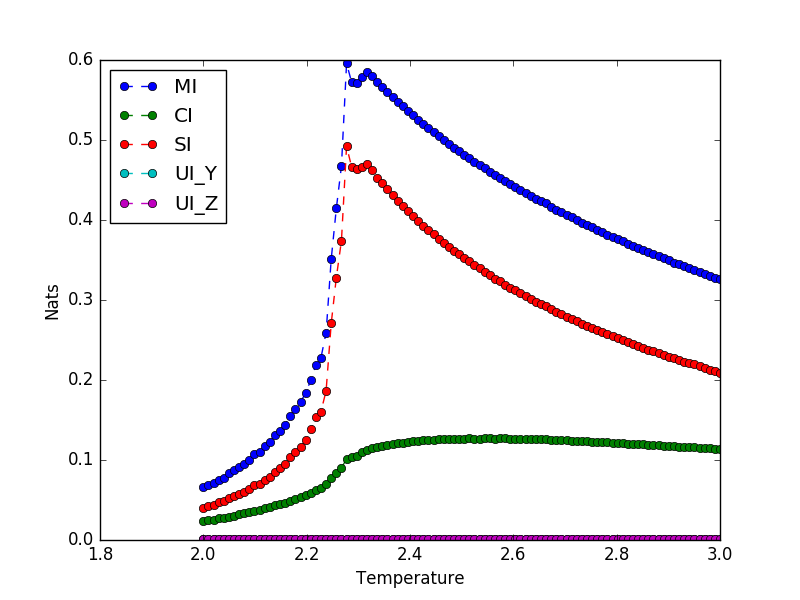
\includegraphics[width=.9\textwidth]{ising-64-pid-4-nbs}
\caption{Average mutual information and PID terms (with all random neighbors considered as inputs) of a 64x64 lattice Ising model evaluated at 102 temperature points spaced evenly over the interval [2.0, 3.0].}
\label{fig:ising-64-pid-4-nbs}
\end{center}
\end{figure}

The results of measuring PID terms when all neighboring sites are considered as inputs to the center site are illustrated in figure \ref{fig:ising-64-pid-4-nbs}. Both mutual and shared information again peak at $T \approx 2.772$. Complementary information peaks at $T \approx 2.5148$, a little nearer to the phase transition than was the case when the lattice size was twice the size (figure \ref{fig:ising-128-pid-4-nbs}). This observation validates that the peak in synergy does not gradually move nearer to the phase transition with increases lattice sizes, ensuring that it is a general property of the model, independent of the lattice size.

\subsection{Elementary cellular automata}

In figure \ref{fig:eca-pid-char}, all 88 inequivalent elementary cellular automata have been depicted based on their partial information decomposition terms. Each point represents a single rule, and the points are colored according to their Wolfram's class. Because there are 4 terms in PID, making their joint visualization on a single plot impossible, principal component analysis was used to project the 4-dimensional PID vectors into 3-dimensional space. It is important to explicitly mention that some "points" in the plot are actually clusters of several rules, but due to their almost identical PID terms, they overlap with each other, yielding a single visual mark on the plot.  For example, the cluster numbered as $1$ appears to be a single point, but there are actually 5 different rules depicted at this location.   

\begin{figure} [!h]
\begin{center}
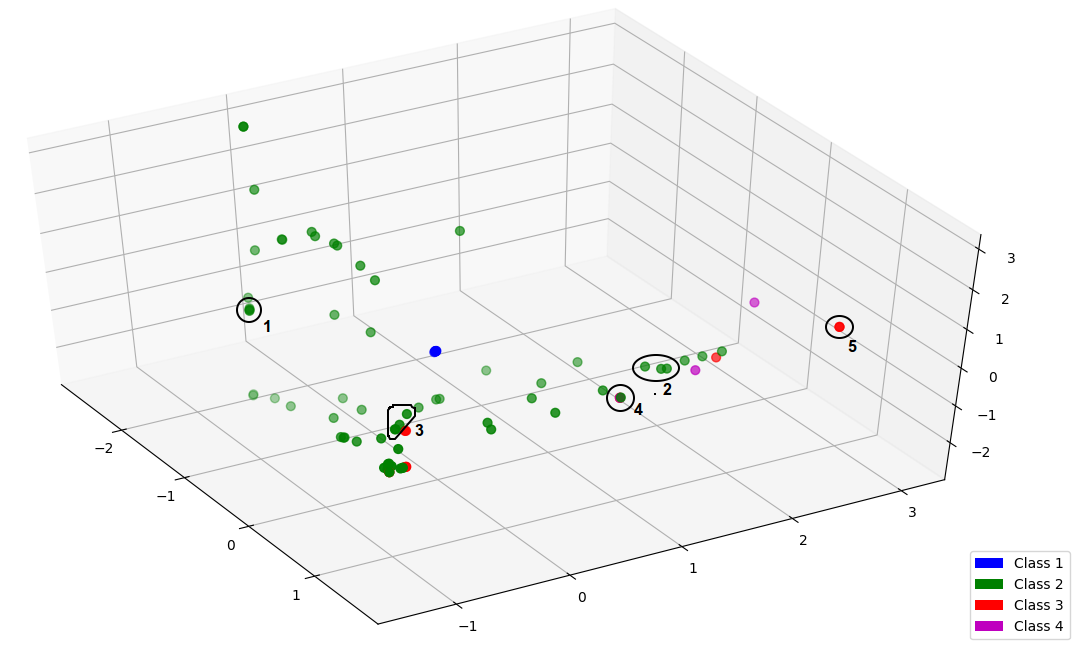
\includegraphics[width=.9\textwidth]{eca-pid-characterization}
\caption{All 88 inequivalent cellular automata positioned on a 3 dimensional space according to their information distribution. The automata are coloured based on their Wolfram's class. Some of the clusters of rules are highlighted and numbered, so that they can be referred to in the text.}
\label{fig:eca-pid-char}
\end{center}
\end{figure}

From the figure, it can be seen that the rules corresponding of Wolfram's class I are all clustered together in a single location separate from the rest of the automata. This is natural, as these class I rules quickly converge to a homogeneous all-white state, such that there is no uncertainty left in the system. In an all-white state, the entropy of the system is 0, yielding mutual information and accordingly, all the PID terms to be 0 as well. While various other cluster appear, they do not correspond well to Wolfram's other 3 classes, meaning that there is no straighforward relationship between Wolfram's classification and the information distribution in elementary cellular automata. 

\begin{figure} [!h]
\begin{subfigure}{.5\textwidth}
  \centering
  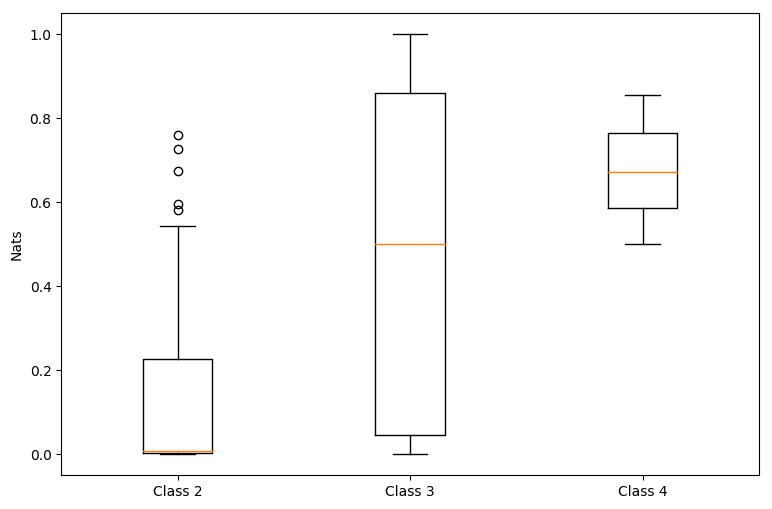
\includegraphics[width=.9\linewidth]{eca-box-ci}
  \caption{Complementary information.}
  \label{fig:eca-box-ci}
\end{subfigure}%
\begin{subfigure}{.5\textwidth}
  \centering
  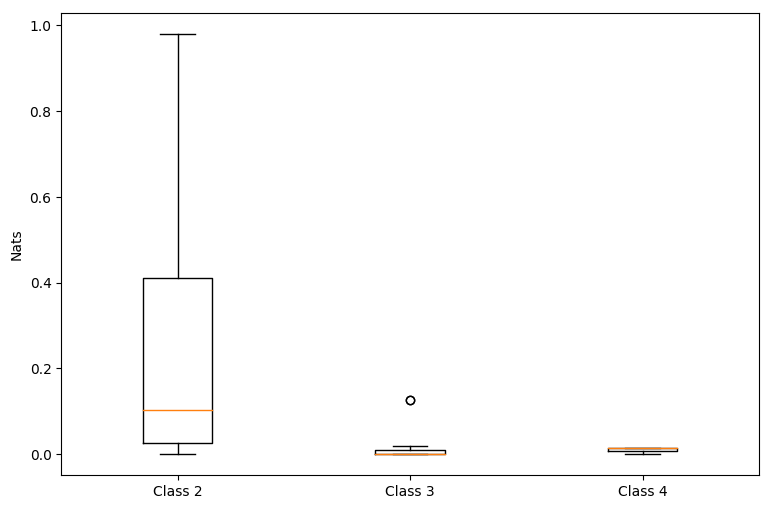
\includegraphics[width=.9\linewidth]{eca-box-si}
  \caption{Shared information.}
  \label{fig:eca-box-si}
\end{subfigure}
\begin{subfigure}{.5\textwidth}
  \centering
  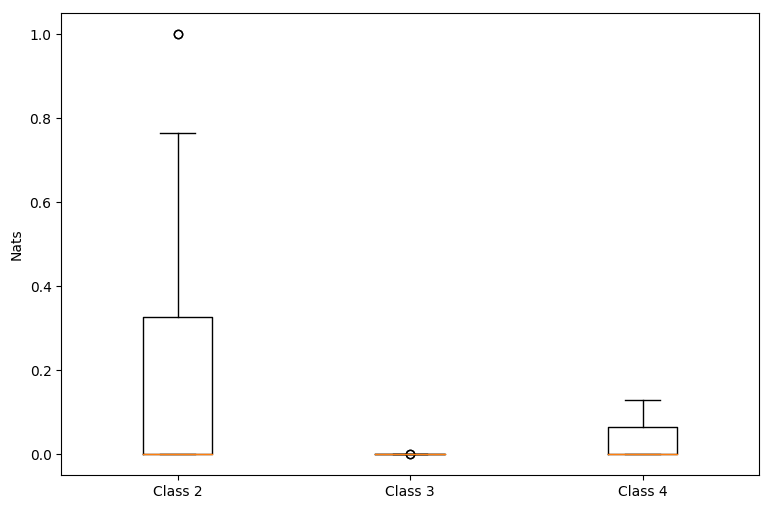
\includegraphics[width=.9\linewidth]{eca-box-ui-y}
  \caption{Unique information of the cell itself.}
  \label{fig:eca-box-ui-y}
\end{subfigure}
\begin{subfigure}{.5\textwidth}
  \centering
  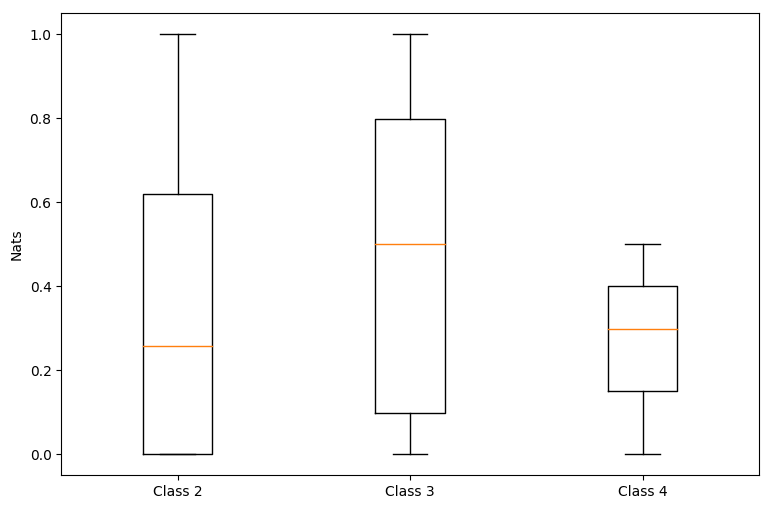
\includegraphics[width=.9\linewidth]{eca-box-ui-z}
  \caption{Unique information of the neighbors.}
  \label{fig:eca-box-ui-z}
\end{subfigure}
\caption{Boxplots representing the values of specific PID terms of cellular automata belonging to Wolfram's classes II, III and IV.}
\label{fig:eca-boxplots}
\end{figure}

The last claim is further justified by figure \ref{fig:eca-boxplots}, which shows the distribution of PID values across Wolfram's classes. From panel \ref{fig:eca-box-ci} it can be seen that in general, the synergy goes up when the complexity of the automata in terms of Wolfram's classification increases. However, there are many outliers in the second class and the variance of the third class is extremely high, making it hard to further draw any specific conclusions. On average, shared information seems to be higher in class 2 automata, while it is almost 0 for the majority of class 3 and 4 automata. Focusing on the last two panels (figures \ref{fig:eca-box-ui-y} and \ref{fig:eca-box-ui-z}), it is evident that two neighbors at the previous timestep have more information about a cell's value at this timestep than its own previous value does. Intuitively, this should indeed hold, since having two sources of information is usually better than having just one. 

Coming back to figure \ref{fig:eca-pid-char} and anlalysing some specific clusters, it becomes apparent that the PID is rather oblivious of the intuitive computational characteristics of elementary cellular automata that Wolfram's classification is based on. For example, it does not capture the complex long-term interactions between various dynamical structures that are important in terms of computation, but happen so infrequently that their influence on the overall probability 	distribution is minimal. Instead, the PID terms seem to depend heavily on the specific local details of the emergent repeating, ubiquituous patterns in the space-time diagrams of cellular automata. To justify this conjecture, some specific examples of clusters are discussed in detail below. 

\begin{figure} [!h]
\begin{subfigure}{.5\textwidth}
  \centering
  
\includegraphics[width=.9\linewidth]{rule6}
  \caption{Rule 6.}
  \label{fig:rule6}
\end{subfigure}%
\begin{subfigure}{.5\textwidth}
  \centering
  
\includegraphics[width=.9\linewidth]{rule38}
  \caption{Rule 38.}
  \label{fig:rule38}
\end{subfigure}
\begin{subfigure}{.5\textwidth}
  \centering
  
\includegraphics[width=.9\linewidth]{rule134}
  \caption{Rule 134.}
  \label{fig:rule134}
\end{subfigure}
\begin{subfigure}{.5\textwidth}
  \centering
  
\includegraphics[width=.9\linewidth]{rule24}
  \caption{Rule 24.}
  \label{fig:rule24}
\end{subfigure}
\begin{subfigure}{.5\textwidth}
  \centering
  
\includegraphics[width=.9\linewidth]{rule130}
  \caption{Rule 130.}
  \label{fig:rule130}
\end{subfigure}
\begin{subfigure}{.5\textwidth}
  \centering
  
\includegraphics[width=.9\linewidth]{rule152}
  \caption{Rule 152.}
  \label{fig:rule152}
\end{subfigure}
\caption{Space-time diagrams of various elementary cellular automata belonging to Wolfram's class II. The first 3 automata from the top belong to cluster 2 in figure \ref{fig:eca-pid-char}, while the remaining rules are from cluster 3.}
\label{fig:eca-diagonal-rules}
\end{figure}

In figure \ref{fig:eca-diagonal-rules}, the space-time diagrams of 6 different rules are depicted, where the dynamics were generated using random initial states. These automata all belong to Wolfram's second class, because they quickly converge into a repetitive state. The diagrams look very alike visually as well, containing densely populated diagonal lines. It would not be unreasonable to expect these rules to be clustered together in figure \ref{fig:eca-pid-char}. Interestingly, however, these rules are partitioned into 2 different clusters that are spaced far apart from each other. In particular, the first 3 rules depicted (rules 6, 38 and 134) appear in cluster 2, while the remaining automata (rules 24, 130, 152) belong to cluster 3. At first glance, this partitioning might be rather confusing, but the conundrum becomes apparent when one zooms in on the space-time diagrams. As can be seen from figure  \ref{fig:eca-diagonals-zoomed}, the intricate structure of the diagonal lines is different between rules 6 and 130. It turns out that rules 6, 38 and 134 all have diagonal lines that are composed of small "inverted L" type blocks, while the diagonals of rules 24, 130 and 152 are much simpler, having a thickness of just a single cell. 

\begin{figure} [!h]
\begin{subfigure}{.5\textwidth}
  \centering
  
\includegraphics[width=.9\linewidth]{rule6-zoomed}
  \caption{Rule 6.}
  \label{fig:rule6-zoomed}
\end{subfigure}%
\begin{subfigure}{.5\textwidth}
  \centering
  
\includegraphics[width=.9\linewidth]{rule130-zoomed}
  \caption{Rule 130.}
  \label{fig:rule130-zoomed}
\end{subfigure}
\caption{Zoomed space-time diagrams of rules 6 (figure \ref{fig:rule6})and 130 (figure \ref{fig:rule130}).} 
\label{fig:eca-diagonals-zoomed}
\end{figure}

To better understand why the specific details of the diagonals yield a radical change in the PID terms, a closer quantitative look at the PID of the rules under discussion is in order. The mutual information of all of the 6 rules is almost exclusively divided between synergy and the unique information provided by the neighbors, leaving the reminaing PID terms close to 0. The first 3 rules each have roughly about $0.55$ nats of synergy and $0.25$ nats of unique information. In contrast, the remaining 3 rules have no complementary information, but their neighbors have about twice as much unique information about the cell's next state, approximately $0.62$ nats each. Thus, almost all of the information in the systems with simpler diagonals is provided uniquely by the neighbors of a site. 

The former numeric observations are not surprising, because looking at the dynamics of rule 6 from figure \ref{fig:rule130-zoomed}, the new states are almost always uniquely determined by the neighbors alone. Indeed, the ubiquituous white background arises mainly because if the right neighbor of a cell is white, this cell's next value will also be white. If, however, the left neighbor is white and the right is black, the cell's next state will be black. The latter relationship produces the diagonals. In case of rule 6, there is a lot more synergy in the system, because neither the cell's previous state or the neighbors are able to produce the complex "reversed L" shaped diagonals alone. The rather high unique information comes from the fact that the left neighbor being black completely determines that the cell's value will be white in the next step. 

\begin{figure} [!h]
\begin{subfigure}{.5\textwidth}
  \centering
  
\includegraphics[width=.9\linewidth]{rule154}
  \caption{Rule 154 (Wolfram's class 2).}
  \label{fig:rule154}
 \end{subfigure}%
\begin{subfigure}{.5\textwidth}
  \centering
  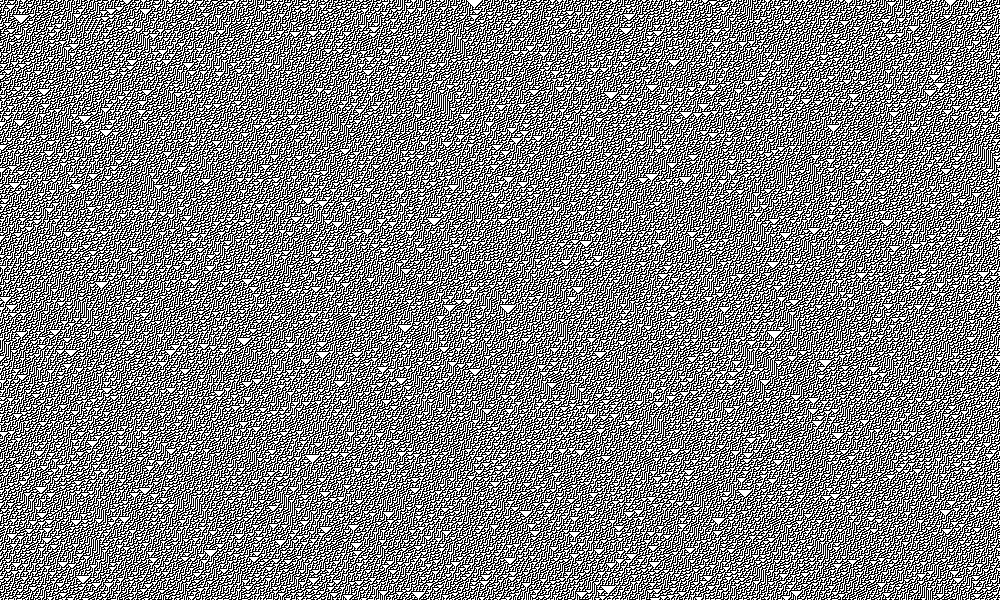
\includegraphics[width=.9\linewidth]{rule30}
  \caption{Rule 30 (Wolfram's class 3).}
  \label{fig:rule30}
\end{subfigure}
\begin{subfigure}{.5\textwidth}
  \centering
  
\includegraphics[width=.9\linewidth]{rule45}
  \caption{Rule 45 (Wolfram's class 3).}
  \label{fig:rule45}
\end{subfigure}
\begin{subfigure}{.5\textwidth}
  \centering
  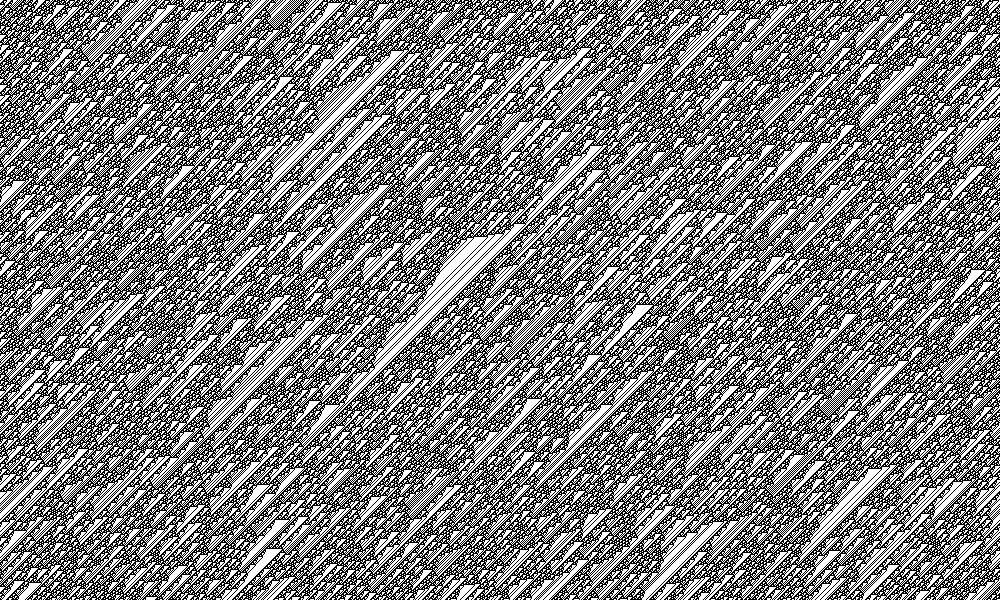
\includegraphics[width=.9\linewidth]{rule106}
  \caption{Rule 106 (Wolfram's class 4).}
  \label{fig:rule106}
\end{subfigure}
\caption{Space-time diagrams of elementary cellular automata belonging to cluster 4 in figure \ref{fig:eca-pid-char}.}
\label{fig:eca-complex-rules}
\end{figure}

Some other clusters are not as straightforward to analyse, but nevertheless, in many cases it is still possible to give some intuitive justifications of the characterization that the PID has produced. For example, figure \ref{fig:eca-complex-rules} depicts the rules in cluster 4, which all have exactly $0.5$ nats of synergy and $0.5$ nats of unique information from the neighbors. While the automata look rather different from the distance, zooming into the lattices again reveals the similarities. Looking at the zoomed space-time diagrams in figure \ref{fig:eca-complex-rules-zoomed}, it can be seen that what the automata under observation have in common is that they all contain rather complex stairway-like structures travelling from the upper right to the lower left.

\begin{figure} [h]
\begin{subfigure}{.5\textwidth}
  \centering
  
\includegraphics[width=.9\linewidth]{rule154-zoomed}
  \caption{Rule 154.}
  \label{fig:rule154-zoomed}
 \end{subfigure}%
\begin{subfigure}{.5\textwidth}
  \centering
  
\includegraphics[width=.9\linewidth]{rule30-zoomed}
  \caption{Rule 30.}
  \label{fig:rule30-zoomed}
\end{subfigure}
\begin{subfigure}{.5\textwidth}
  \centering
  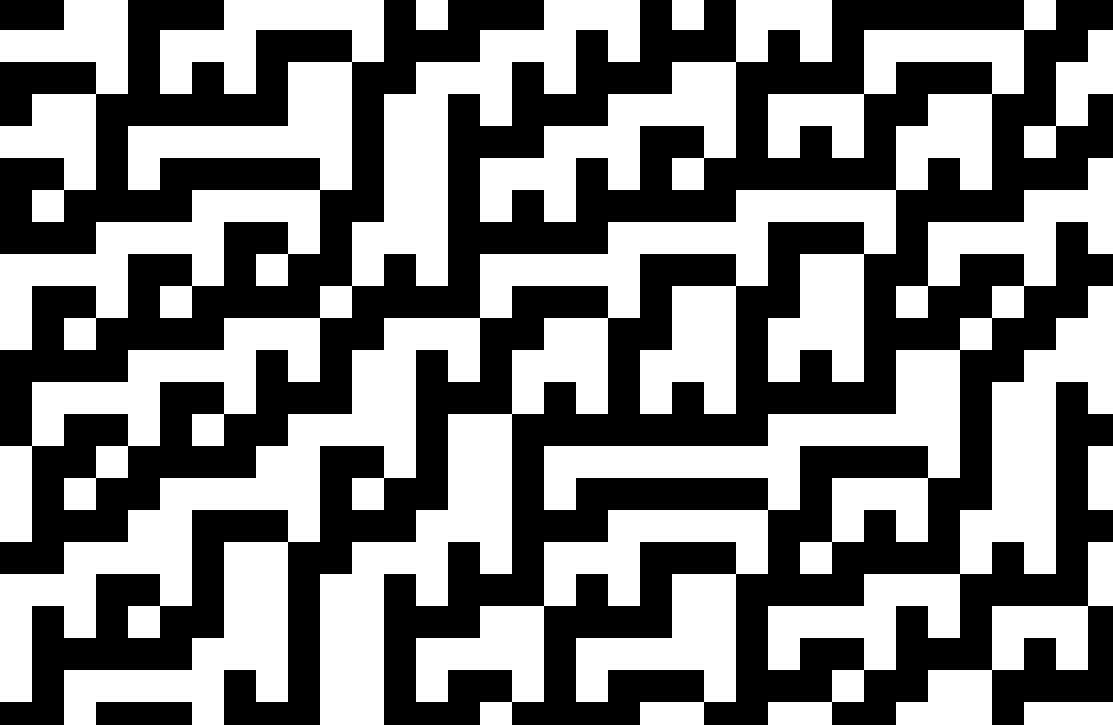
\includegraphics[width=.9\linewidth]{rule45-zoomed}
  \caption{Rule 45.}
  \label{fig:rule45-zoomed}
\end{subfigure}
\begin{subfigure}{.5\textwidth}
  \centering
  
\includegraphics[width=.9\linewidth]{rule106-zoomed}
  \caption{Rule 106.}
  \label{fig:rule106-zoomed}
\end{subfigure}
\caption{Zoomed space-time diagrams of the automata plotted in figure \ref{fig:eca-complex-rules}.}
\label{fig:eca-complex-rules-zoomed}
\end{figure}

Another noteworthy collection of rules is cluster 5, which consists  of 3 automata that Wolfram has classified as chaotic. All the automata belonging to this cluster have 1 nat of mutual information, which is all exclusively provided by complementary information. The cluster is interesting because it shows that at least for some subset of automata, their qualitative characterization coincides with the quantitative one provided by the PID. 

\newpage
\section{Discussion}

This chapter starts by putting the results obtained in the two complex systems into a larger context and by discussing their implications.  The possibility of analysing other dynamical complex systems with the information-theoretic tools used in this thesis is crticially examined in the second section. The chapter concludes with numerous suggestions for further work. 

\subsection{Implications of the results}

In \cite{barnett-ising}, it is shown that global transfer entropy peaks in the disorder phase in the Ising model, just before the phase transition. In other words, transfer entropy was found to be able predict the order-disorder transition before it actually takes place. In a subsequenet commentary discussing this work \cite{inf-flow-ising-commentary}, Lionel Barnett, one of the authors of the paper, argues that this result might also generalize to other real-world dynamical complex systems that undergo phase transitions. The practical importance of this could be immense. Among other things, one can imagine it being used to predict imminent epileptic seizures and financial market crashes in advance. 

In this thesis, it was found that one of the PID terms, complementary information, also obtains a maximum in the disorder regime in the Ising system. Taking the commentary by Barnett into account, it would be worthwhile to study various real-world systems in terms of partial information decomposition. In particular, it would be interesting to measure the synergy between various components with the hope of predicting the arising phase transition  in advance.

As for elementary cellular automata, the obtained characterization of the rules based on the PID terms is a great addition to Wolfram's classification. While Wolfram's 

\subsection{Limitations}

The two complex systems analysed in this thesis have an important property in common that makes their investigation with the PID estimator convenient, not to say possible. First, they are both binary, meaning that the individual elements of the systems can only be in two different states. Second, in both systems, each local part of the model is directly influenced by only a handful of other agents. Indeed, in the Ising model, the energy of a single site depends only on the spins of its 4 immediate neighbors, while the next value of a cell in elementary cellular automata is determined by the 3 cells in its local neighborhood. What follows is a discussion of why both of these characteristics are paramount to successful analysis of information distribution in complex systems. 

First, the systems being binary, or more generally, discrete with relatively few possible states, ensures that the number of rows in the probability distribution that the PID numerical estimator takes as input is relatively small. The number of rows of the distribution increases polynomially in the number of states of the random variables that it contains. For example, a distribution with 3 random variables with 20 possible states would have 8000 rows. Such a large distribution would be unmanagable for the numerical estimator, which is able to maximally handle distributions with roughly 2000 rows. This problem also arises when the analysed system has continuous elements, since one must approximate the continuous functions using discretization, in particular, by dividing the continuous signal into a finite number of different states. To analyse the performance of the estimator, a multivariate Gaussian probability distribution was generated, discretized, and fed into the estimator. It was empirically validated that the estimator terminates and gives a solution in reasonable time (under half an hour of processing) when the level of discretization is less than 14.   

Second, the systems having few directly interdependent components again ensures that the number of rows in the distributions is relatively small, the latter increasing polynomially in the number of random variables that the 3 random vectors contain. There is, however, an even more fundamental problem that has nothing to do with the numerical estimator, but rather with the fact that the PID mathematical framework has currently been developed for 2 logical input sets only. In particular, if the number of inputs in the system grows, and they are not logically partitionable into two distinct sets, it becomes increasingly hard to reasonably choose the two subsets of input channels. Even if the input space is composed of two logical sets, taking only a small subset of components from each might not yield desirable results. This is because  there is exponentially many ways to choose the subsets with respect to each other, and there is often no straightforward way to know which configuration is the "right" one. 

To better understand the argument put forth in the last paragraph, it is instructive to look at the results of another preliminary experiment that was carried out as part of this thesis. In particular, the average information distribution between the nodes in a feedforward neural network was analysed while it was trained on a classification task. The model consisted of 2 hidden units, each containing 300 neurons. While such models usually have continuous activation functions, it is not feasible to discretize these continuous signals with fine enough granularity without making their analysis with the estimator unfeasible. Thus, binary activations were used in the hidden layers of the network, as introduced in \cite{binary-nets}. The output layer of the network consisted of softmax units. The network was trained on the MNIST handwritten digit database \cite{mnistlecun} for 150 epochs. Figure \ref{fig:neural-net-loss} depicts the training and validation learning curves of this classifier.

\begin{figure} [h]
\begin{center}
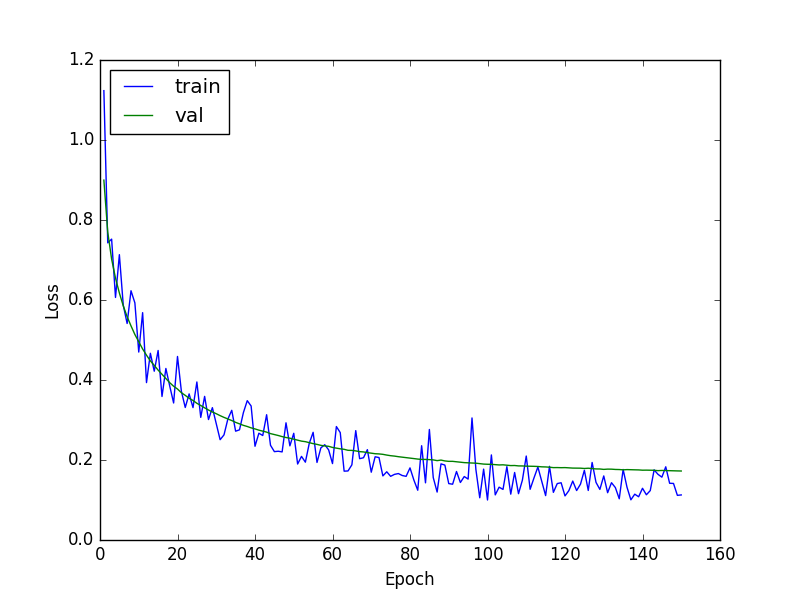
\includegraphics[width=.9\textwidth]{neural-net-loss}
\caption{Learning curves of a neural network that was trained to classify MNIST handwritten digits.}
\label{fig:neural-net-loss}
\end{center}
\end{figure}

In neural networks, the parameters are initialized randomly, and as a result, the model's loss is initially rather high, as can also be seen from figure \ref{fig:neural-net-loss}. During training, the weights of the network are incrementally tweaked in such a way that the performance of the model increases. Thus, neural networks can be thought of as exhibiting a phase transition, where the weights gradually move from an unorganized random state to an organized one. The training or validation loss represents the order parameter, with higher values meaning that the system has more disorder, and vice versa. Insipired by the results obtained from analysing the Ising model, the neural network under discussion was investigated with the PID numerical estimator with the hope of discovering interesting behaviour of the PID functionals near the order-disorder phase. More specifically, one could expect some interesting behaviour of some of the PID terms between the epochs 15 and 50, because it is during this time that the derivative of the loss function undergoes the most rapid change.

To estimate the information distribution in the system, 200 triplets were taken for analysis. For each triplet, the two inputs were taken to be two random nodes from the last hidden layer of the network, and the output was taken to be the true target decimal value. The 200 probability distributions were subsequently fed into the PID numerical estimator and the results averaged. This procedure was repeated for each epoch, but the 200 triplets remained the same thorughout the experiment. The obtained PID functionals are illustrated in figure \ref{fig:neural-net-pid}.

\begin{figure} [h]
\begin{center}
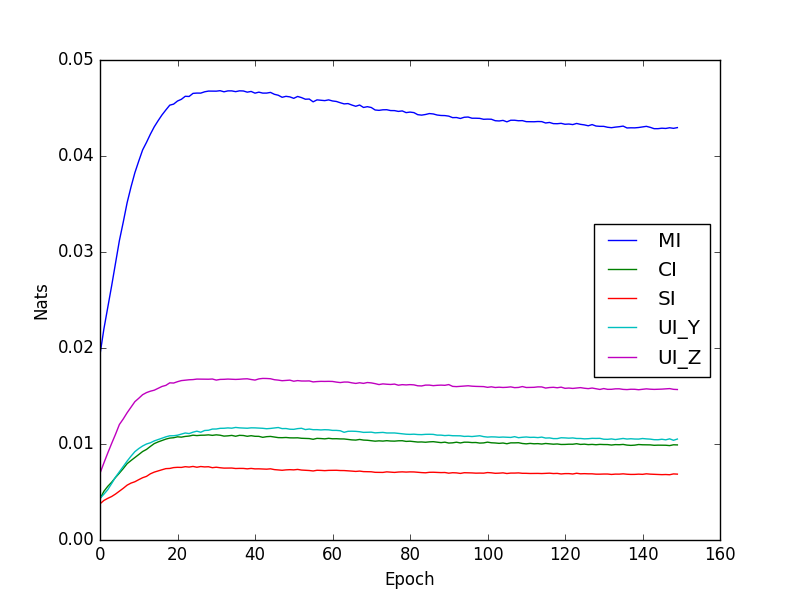
\includegraphics[width=.9\textwidth]{neural-net-pid}
\caption{The average information distribution between the nodes in a feedforward neural network.}
\label{fig:neural-net-pid}
\end{center}
\end{figure}

From figure \ref{fig:neural-net-pid}, it can be seen that the mutual information behaves similar to the reflection of the training loss over the horizontal axis. This agrees with the observation made in \cite{it-neural-nets}, in which the mutual information between the neurons in a toy neural network was measured during training. Looking at the PID terms, one can see that the unique information terms follow the mutual information curve almost exactly, and that complementary and redundant information terms are both essentially 0. It is the author's belief that the PID terms are rather uninteresting largely because the inputs do not come from 2 logically distinct subsystems. Every neuron in the last layer has 299 neighbors, and there is no fundamental reason to prefer one neighbor over the other. One might argue that no natural partitioning exists in the case of the Ising model as well. However, in the latter system, a site depended only on 4 of its neighbors, making the problem much less pressing. 

\subsection{Future work}

There are various promising research directions in the domain of partial information decomposition itself. First, the estimator could be improved in various ways. Most notably, the optimization could be made faster, so that the larger probability distributions would also be possible to analyse. Further, the mathematical framework of partial information decomposition has currently been developed only for the bivariante input case. The general decomposition of multi-variate information remains to be developed. 

In the case of the Ising model, it might be of interest to study how information is distributed between the different parts of the model more theoretically. This would provide some further insight as to why the PID functionals behave as they do in this specifc model. In addition, the results obtained in the Ising system should inspire further research into real-world complex systems in which it would be of importance to predict the occurrence of a phase transition in advance. 

In this thesis, elementary cellular automata were studied, in which by definition, each cell is directly influenced by only 3 cells in its local neighborhood. However, these relatively simple systems are just a special case of a larger class of models, called \textit{1-dimensional cellular automata}, where cells can depend on an arbitrary fixed number of nearby cells. It is up to further work to study the information distribution in cellular automata that are not elementary. \cite{Das1994} used genetic algorithms to discover different rules that are able to perform specific tasks, like classifying whether the majority of cells in the initial configuration have a value of 1. It could worthwhile to study if the information distribution, as measured by the PID terms, is similar in different automata that solve a common task. 

There are many promising research directions when it comes to analysing the information distribution in artificial neural networks. The PID measurements obtained from analysing feedforward neural networks in this thesis were uninteresting largely because there is no natural partitioning of nodes in this model. However, such a partitioning does exist in recurrent neural networks, where each neuron has both bottom-up inputs from the previous layer and lateral contextual inputs from the same layer at the previous timestep. Applying the current numerical estimator to recurrent networks can prove to be difficult, however, as to the author's knowledge, there is no existing work validating that binarizing the activations of a reccurent model yields a reasonable model. 

\newpage
\section*{Conclusion}
\addcontentsline{toc}{section}{Conclusion}

\selectlanguage{english}

\newpage
\bibliographystyle{alpha}
\addcontentsline{toc}{section}{Bibliography}
\bibliography{bachelor-thesis}

\appendix
\pagebreak
\section*{\small Non-exclusive licence to reproduce thesis and make thesis public}


I, Sten Sootla (date of birth: 17th of January 1995),

\begin{tabbing}
\= Xiii\=\kill
\>1. \> herewith grant the University of Tartu a free permit (non-exclusive licence) to:\\\\ 

\>1.1\> 
\begin{minipage}[t]{14.2cm}
reproduce, for the purpose of preservation and making available to the public, including for addition to the DSpace digital archives until expiry of the term of validity of the copyright, and
\end{minipage}
\\\\
\>1.2 
\begin{minipage}[t]{14.2cm}
make available to the public via the web environment of the University of Tartu, including via the DSpace digital archives until expiry of the term of validity of the copyright,\\ 

Analysing information distribution in complex systems\\   

supervised by Raul Vicente Zafra and Dirk Oliver Theis

\end{minipage}\\\\ 
\>2. \>I am aware of the fact that the author retains these rights.\\\\
\>3. \>
\begin{minipage}[t]{14.2cm}
I certify that granting the non-exclusive licence does not infringe the intellectual property rights or rights arising from the Personal Data Protection Act. 
\end{minipage}\\
\end{tabbing}

\noindent
Tartu, dd.mm.yyyy


\end{document}

